\documentclass{article}
\usepackage[utf8]{inputenc}
\usepackage[margin = 0.8in]{geometry}
\usepackage{graphicx}
\usepackage{amsmath, amssymb}
\usepackage{subcaption}
\usepackage{multirow}
\usepackage{mathtools}
\usepackage{float}


\title{RBE502 - Homework Set 7}
\author{Keith Chester}
\date{Due date: October 17 2021}

\begin{document}
\maketitle

\section*{Introduction}

In this assignment, we will be looking at a 2 link robotic arm as depicted in the figure below. We will be designing a feedback linearization controller to stabilize the robotic arm on a desired orientation/position.

\begin{figure}[H]
    \centering
    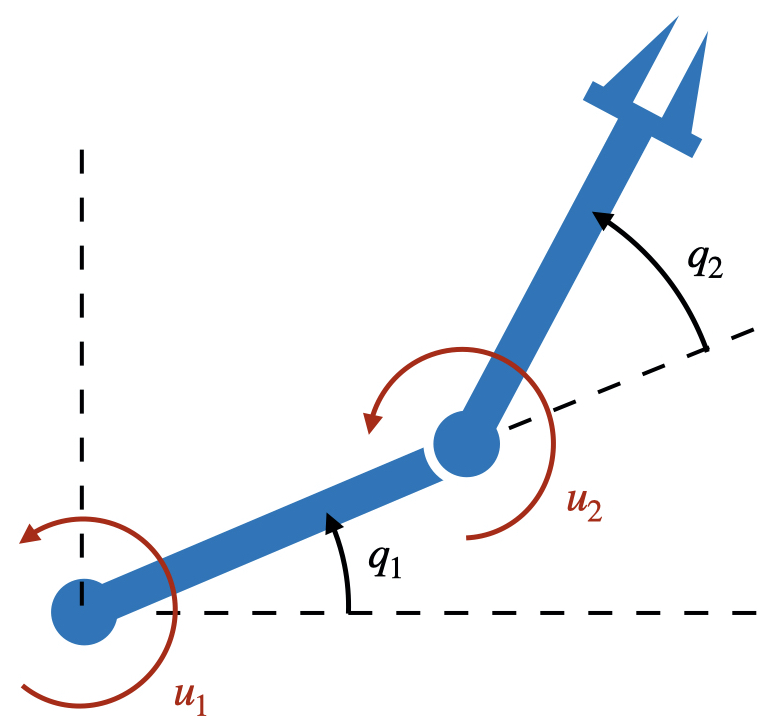
\includegraphics[width = 0.4\textwidth]{figures/2D-rr.001.jpeg}
    \caption{2 link robotic arm}
    \label{fig:robot-arm}
\end{figure}

This arm can be expressed mathematically as a double pendulum system as depicted in the following figure.

\begin{figure}
    \centering
    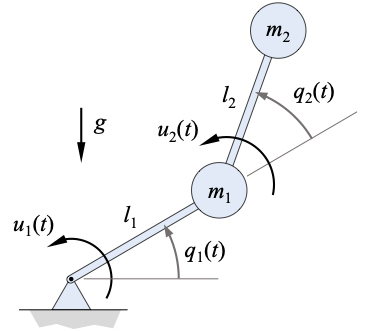
\includegraphics[width=0.4\textwidth]{figures/doublependulum.jpg}
    \caption{Double pendulum system}
    \label{fig:double-pendulum}
\end{figure}

Within this system, we can define $M(q)$, $T(q)$, and $\phi(q, \dot{q})$ as:

\begin{equation}
    M(q) = \begin{bmatrix}
        (m_1 + m_2)l_1^2+m_2*l_2^2+2l_1l_2m_2\cos{q_2} & m_2l_2(l_1\cos{q_2}+l_2) \\
        m_2l_2(l_1\cos{q_2}+l_2) & m_2l_2^2
    \end{bmatrix}
\end{equation}

\begin{equation}
    T(q) = \begin{bmatrix}1 & 0 \\ 0 & 1\end{bmatrix}
\end{equation}

\begin{equation}
    \phi(q) = \begin{bmatrix}
        (m1+m2)gl_1\cos{q_1)+m_2l_2(g\cos(q_1+q_2)-l_1\dot{q}_2(2\dot{q}_1+\dot{q}_2)\sin{q_2})}
        \\
        m_2l_2(l_1\dot{q}_1^2+g\cos{q_1+q_2})
    \end{bmatrix}
\end{equation}

We further define $x = \begin{bmatrix} q_1 & q_2 & \dot{q}_1 & \dot{q}_2 \end{bmatrix}^T$. From this we can compile these equations into a system:

\begin{equation}
    \dot{x} = \begin{bmatrix}
        q \\ \dot{q}
    \end{bmatrix} =
    f(x) + g(x)u
    =
    \begin{bmatrix}
        \dot{q} \\
        -M^{-1}\phi(q, \dot{q})
    \end{bmatrix} + 
    \begin{bmatrix}
        \boldsymbol{0} \\
        M^{-1}T(q)
    \end{bmatrix} u
\end{equation}

From this we can select a desired state, $x_d$, and define the error dynamics as:

\begin{equation}
    \dot{e} = \dot{x}_d - \dot{x} = 0 - f(x) - g(x)u = -f(x_d - e)-g(x_d-e)u
\end{equation}

We further simplify this by defining $f_e(u) = -f(x_d - e)$ and $g_e(u) = -g(x_d-e)$, thus making our final equation $\dot{e}=f_e(e)+g_e(e)u$.

\section*{Part A}

In this section, we are looking to use the error dynamics function and design a feedback linearization control law that reduces our error to zero. We are looking to find the control function $u = \gamma(e)(\sigma(e)-Ke)$ and utilize it to eliminate nonlinear terms.

To this end, we have assigned the following equations for our $\gamma(e)$ and $\sigma(e)$:

\begin{equation}
    \gamma(e) = \begin{bmatrix}
        \boldsymbol{0} \\
        -M(e)T
    \end{bmatrix}
\end{equation}

\begin{equation}
    \sigma(e) = -f_e(e)
\end{equation}


\section*{Part B}

In this section, we now assigned values to constants utilized throughout our system and attempt to calculate a resulting matrix $\boldsymbol{K}$. We'll be utilizing $m_1 = 10 kg$, $m2 = 4kg$, $l_1=1m$, $l_2=2m$, and $g=9.81\frac{m}{s^2}$.

If we set $e=\begin{bmatrix}
    e_1 & e_2 & e_3 & e_4
\end{bmatrix}^T$, then we can solve for $\dot{e}$ utilizing our system of equations above. First, however, we need to define $\boldsymbol{K}$ to be a matrix of several subvalues $k_{i,j}$. Some of these values must be zero'ed out in order to present a solvable system. To do so, we will be utilizing:

\begin{equation}
    K = \begin{bmatrix}
        k_{11}  & k_{12}  & k_{13}  & k_{14} \\
        k_{21}  & k_{22}  & k_{23}  & k_{24} \\
        k_{31}  & 0 & k_{33}  & 0\\
        0 & k_{42}  & 0 & k_{44} 
        \end{bmatrix}
\end{equation}

...and thus, we can solve for $\boldsymbol{K}$:

\begin{equation}
    \dot{e}=f_e(e)+g_e(e)u=f_e(e)+g_e(e)\gamma(e)(\sigma(e)-K_e) = \begin{bmatrix}
        e_3 \\
        e_4 \\
        -e_1 \,k_{31} -e_3 \,k_{33} \\
        -e_2 \,k_{42} -e_4 \,k_{44} 
    \end{bmatrix}
\end{equation}

...to which we can solve for our $\boldsymbol{A}$ matrix, by taking the Jacobian of this result:

\begin{equation}
    A = jacobian(\dot{e}) = \begin{bmatrix}
        0 & 0 & 1 & 0\\
        0 & 0 & 0 & 1\\
        -k_{31}  & 0 & -k_{33}  & 0\\
        0 & -k_{42}  & 0 & -k_{44} 
        \end{bmatrix}
\end{equation}

From here, we can solve the resulting eigenvalues of A to match the given eigenvalues of $\lambda = \{ -1, -2, -3, -4 \}$:

\begin{equation}
    \sigma_{eigenvalues}(\begin{bmatrix}
        0 & 0 & 1 & 0\\
        0 & 0 & 0 & 1\\
        -k_{31}  & 0 & -k_{33}  & 0\\
        0 & -k_{42}  & 0 & -k_{44} 
        \end{bmatrix}) + \begin{bmatrix}
        4 \\ 3 \\ 2 \\ 1
    \end{bmatrix} = 0
\end{equation}

Solving for the specified surviving values of $\boldsymbol{K}$ found within $\boldsymbol{A}$, we find that the valus of $k_{31} = 12$, $k_{33}=7$, $k_{42}=2$, and $k_{44}=3$. Thus our resulting system $\boldsymbol{K}$ is:

\begin{equation}
    \boldsymbol{K} = \begin{bmatrix}
        0 & 0 & 1 & 0 \\
        0 & 0 & 0 & 1 \\
        12& 0 & 7 & 0 \\
        0 & 2 & 0 & 3
    \end{bmatrix}
\end{equation}

\section*{C}

In this section, we will be looking at the system utilizing the $\boldsymbol{K}$ calculated above for different desired orientations $x_d$. We assume that the arm starts in the orientation of $x_0 = \begin{bmatrix}
    0 & 0 & 0 & 0
\end{bmatrix} ^ T $.

\subsection*{I: $x_d = \begin{bmatrix} 0 & \frac{\pi}{2} & 0 & 0 \end{bmatrix}^T$}

\begin{figure}[H]
    \centering
    \begin{subfigure}{0.325\textwidth}
        \centering
        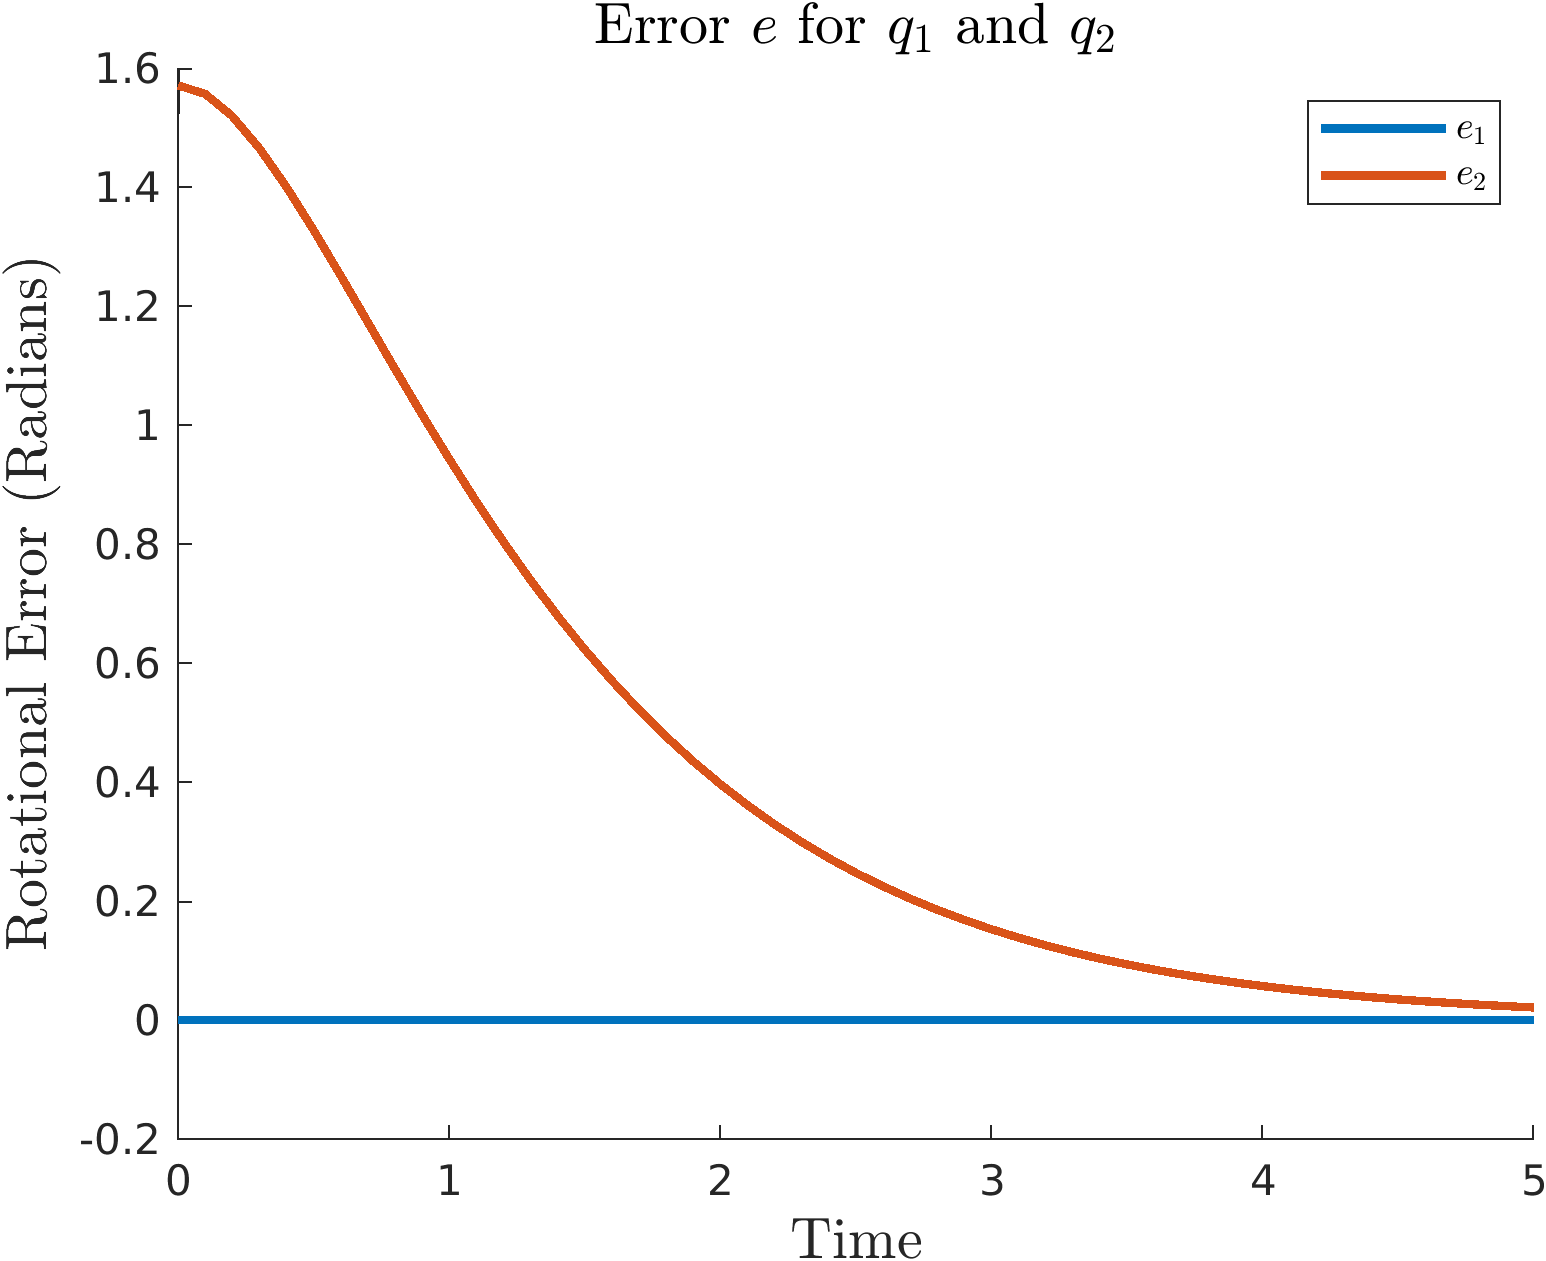
\includegraphics[width = \textwidth]{figures/error-c1.png}
        \caption{Error over time}
    \end{subfigure}
    \begin{subfigure}{0.325\textwidth}
        \centering
        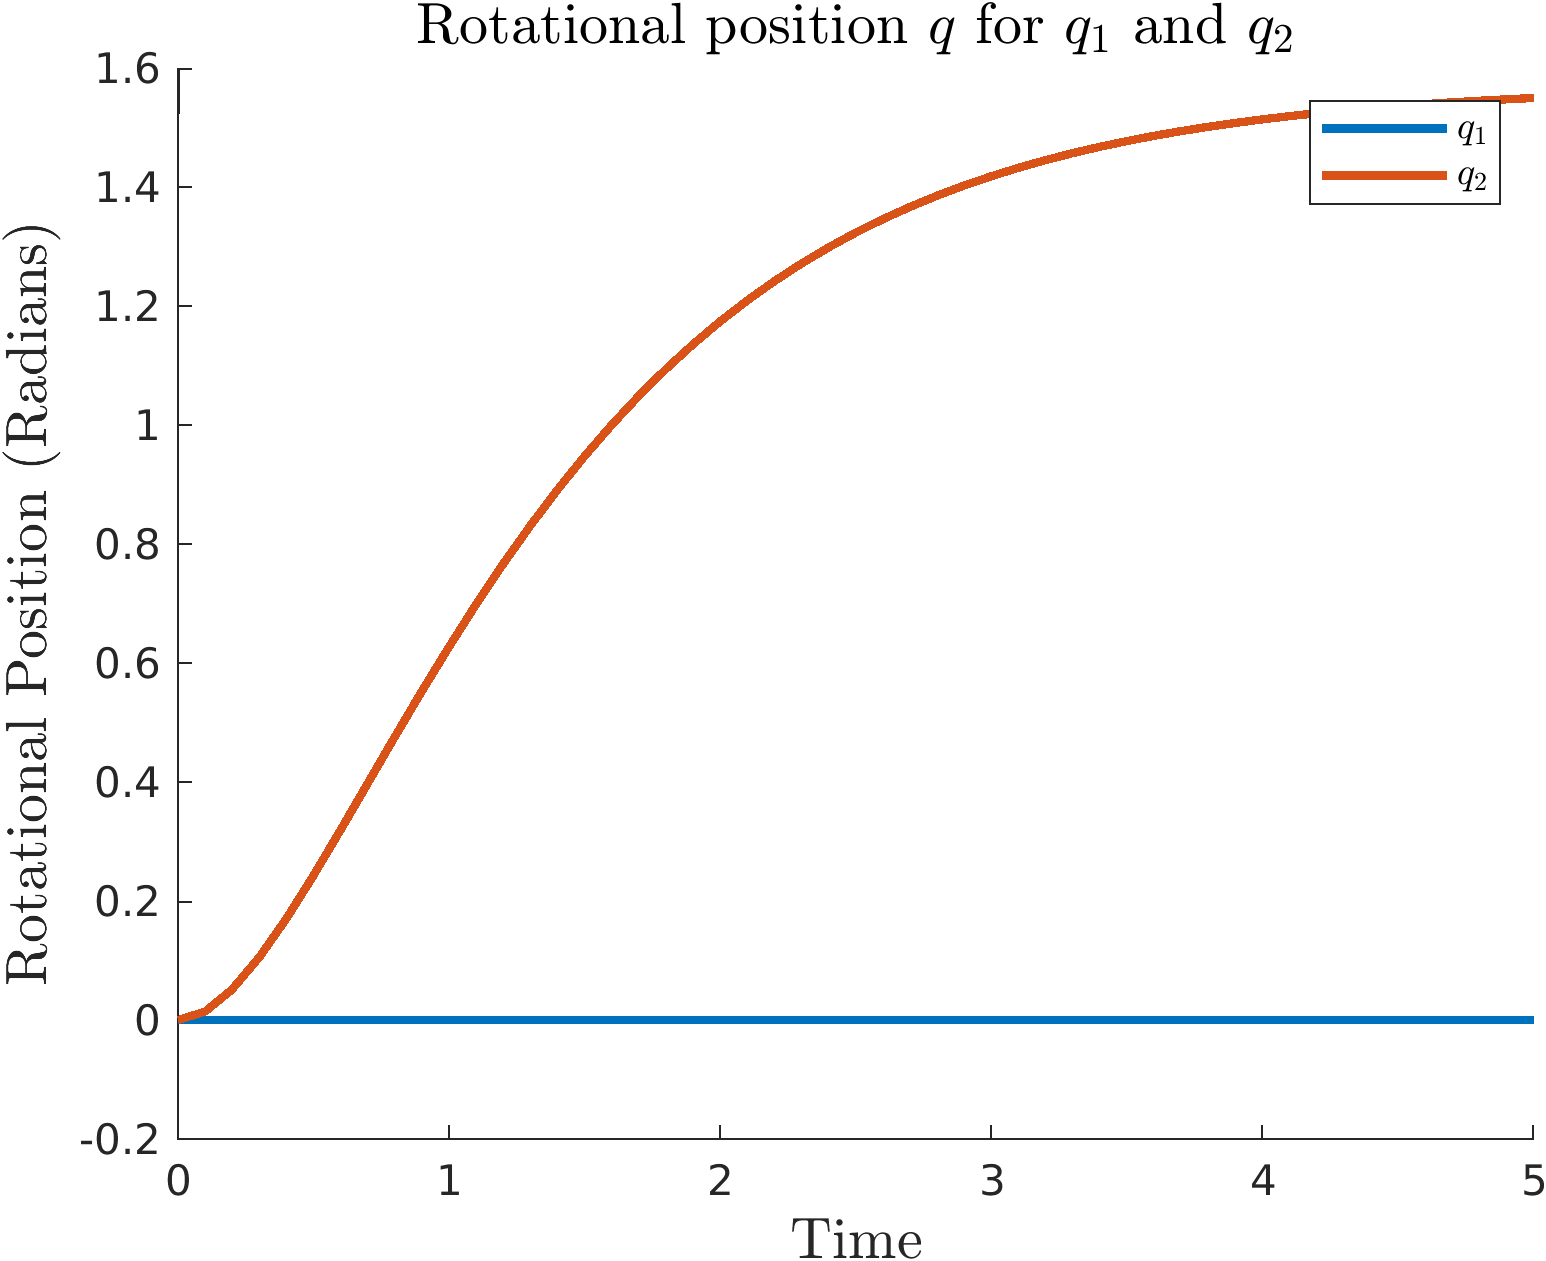
\includegraphics[width = \textwidth]{figures/rotational-position-c1.png}
        \caption{Rotational position over time}
    \end{subfigure}
    \begin{subfigure}{0.325\textwidth}
        \centering
        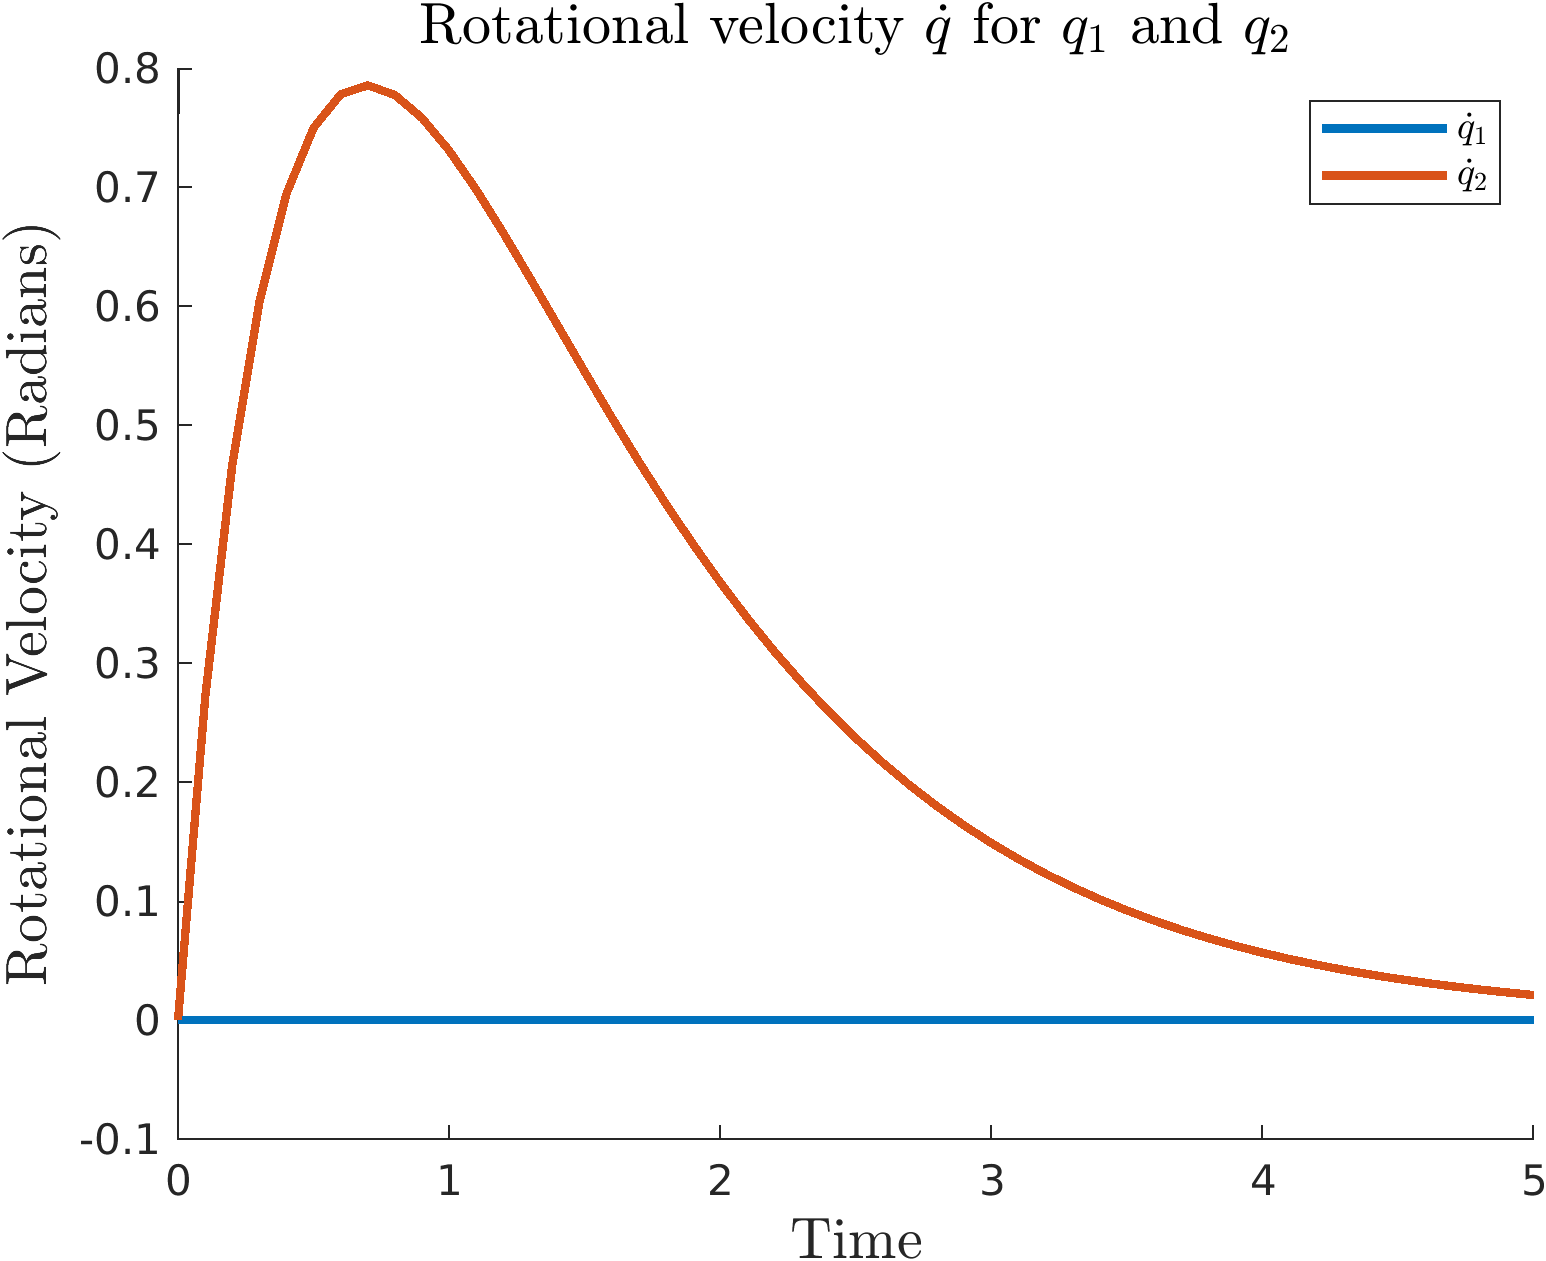
\includegraphics[width = \textwidth]{figures/rotational-velocity-c1.png}
        \caption{Rotational velocity over time}
    \end{subfigure}
    \caption{System response with $x_d=\begin{bmatrix} 0 & \frac{\pi}{2} & 0 & 0 \end{bmatrix}^T$}
    \label{fig:c-1_results}
\end{figure}


\subsection*{II: $x_d = \begin{bmatrix} \frac{\pi}{2} & 0 & 0 & 0 \end{bmatrix}^T$}

\begin{figure}[H]
    \centering
    \begin{subfigure}{0.325\textwidth}
        \centering
        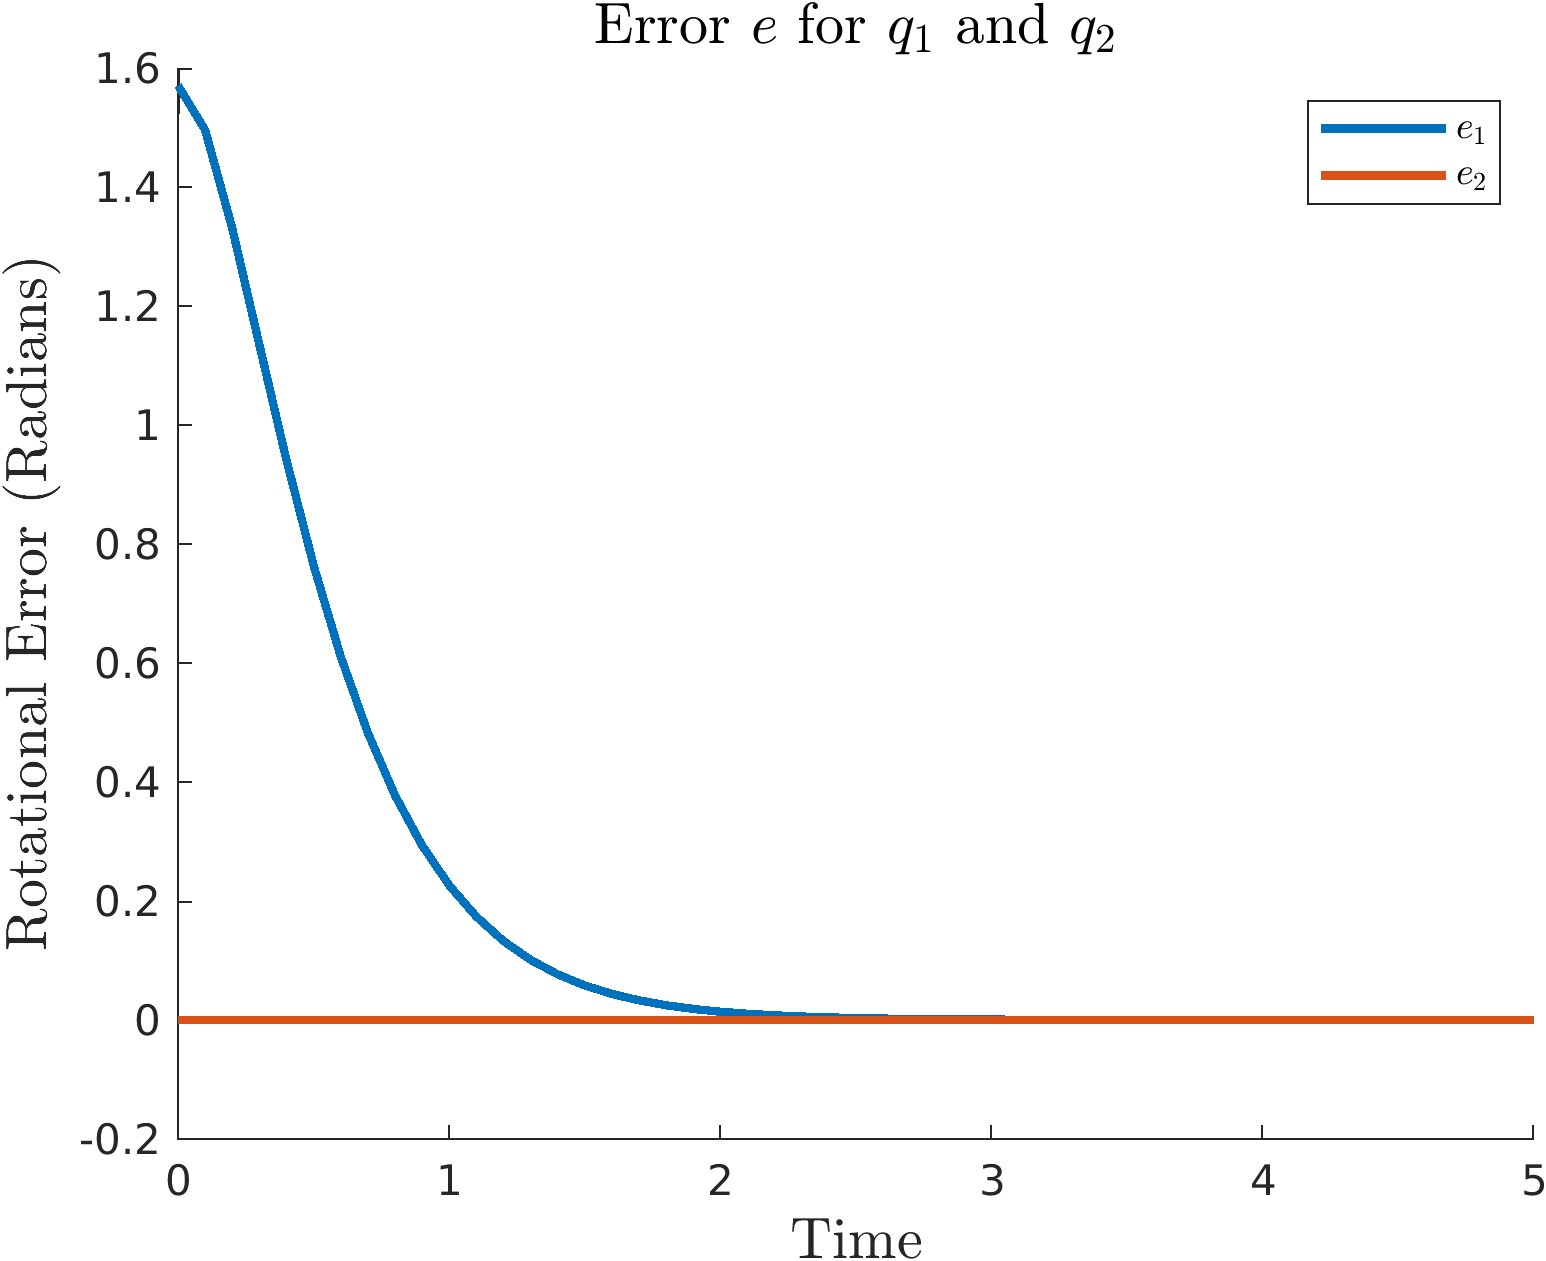
\includegraphics[width = \textwidth]{figures/error-c2.png}
        \caption{Error over time}
    \end{subfigure}
    \begin{subfigure}{0.325\textwidth}
        \centering
        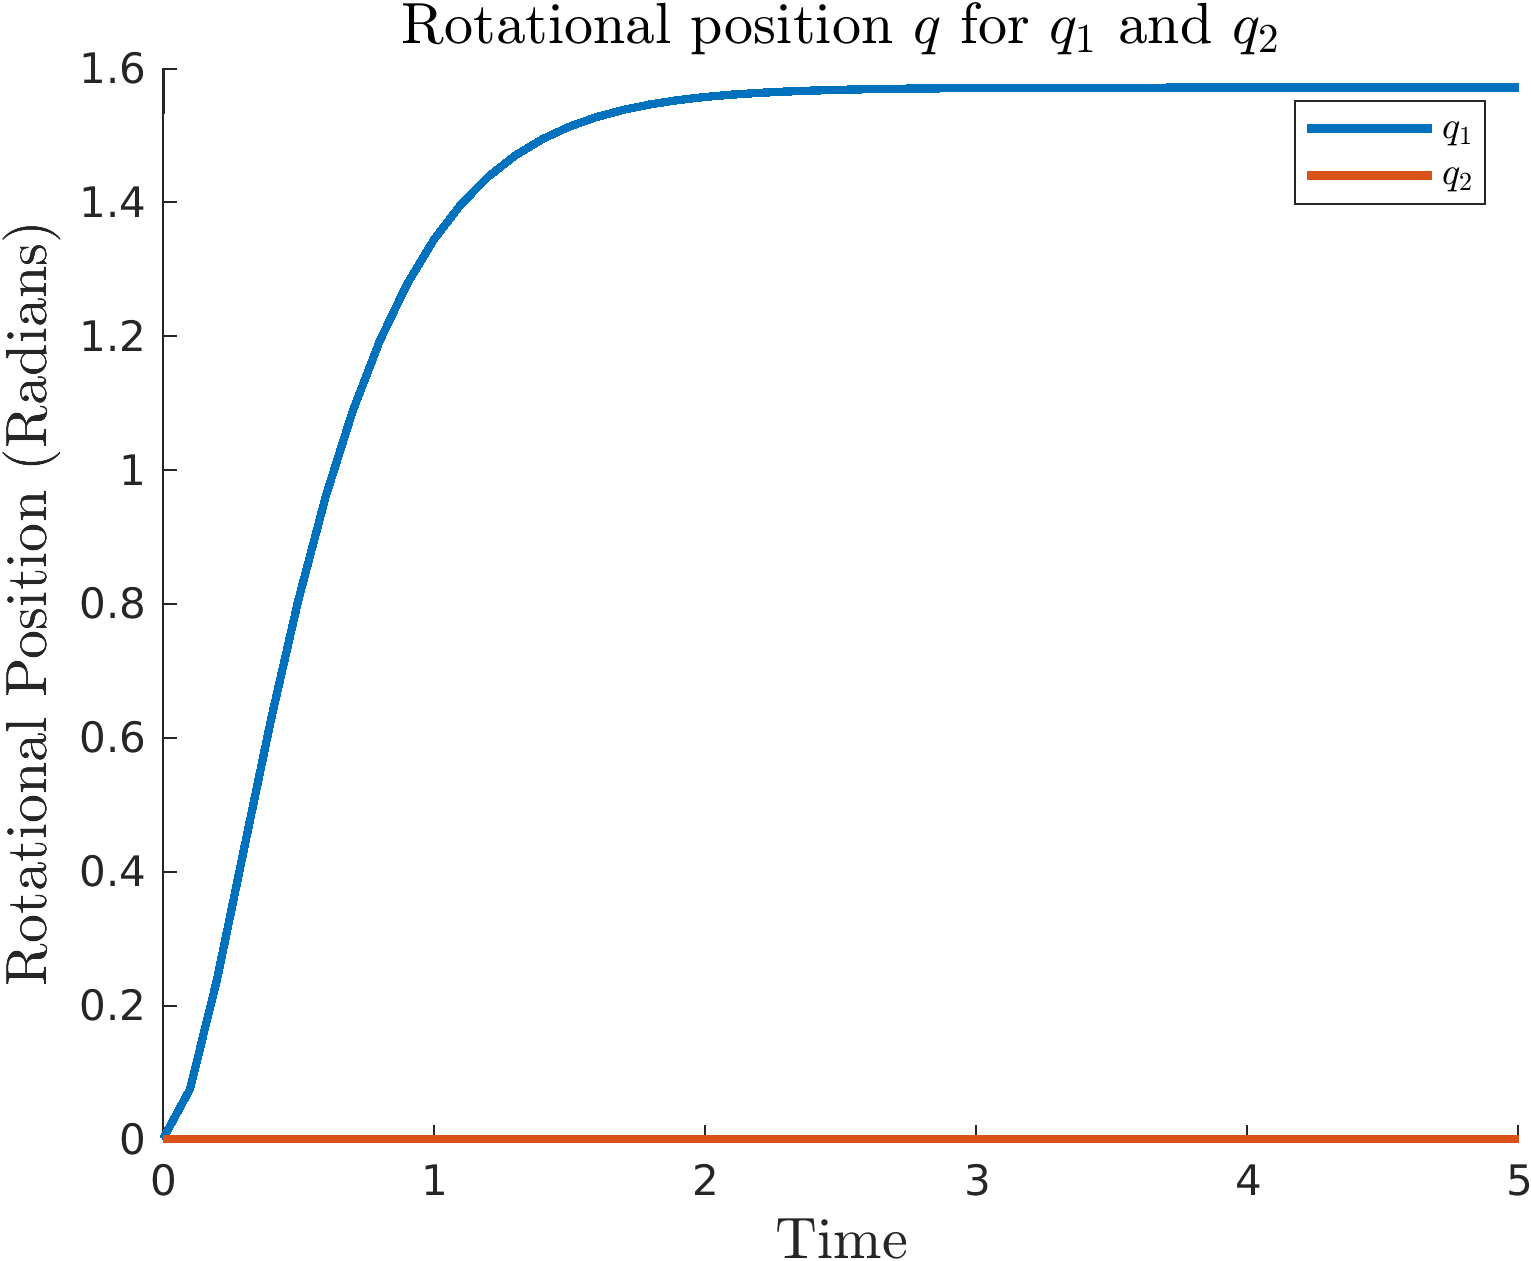
\includegraphics[width = \textwidth]{figures/rotational-position-c2.png}
        \caption{Rotational position over time}
    \end{subfigure}
    \begin{subfigure}{0.325\textwidth}
        \centering
        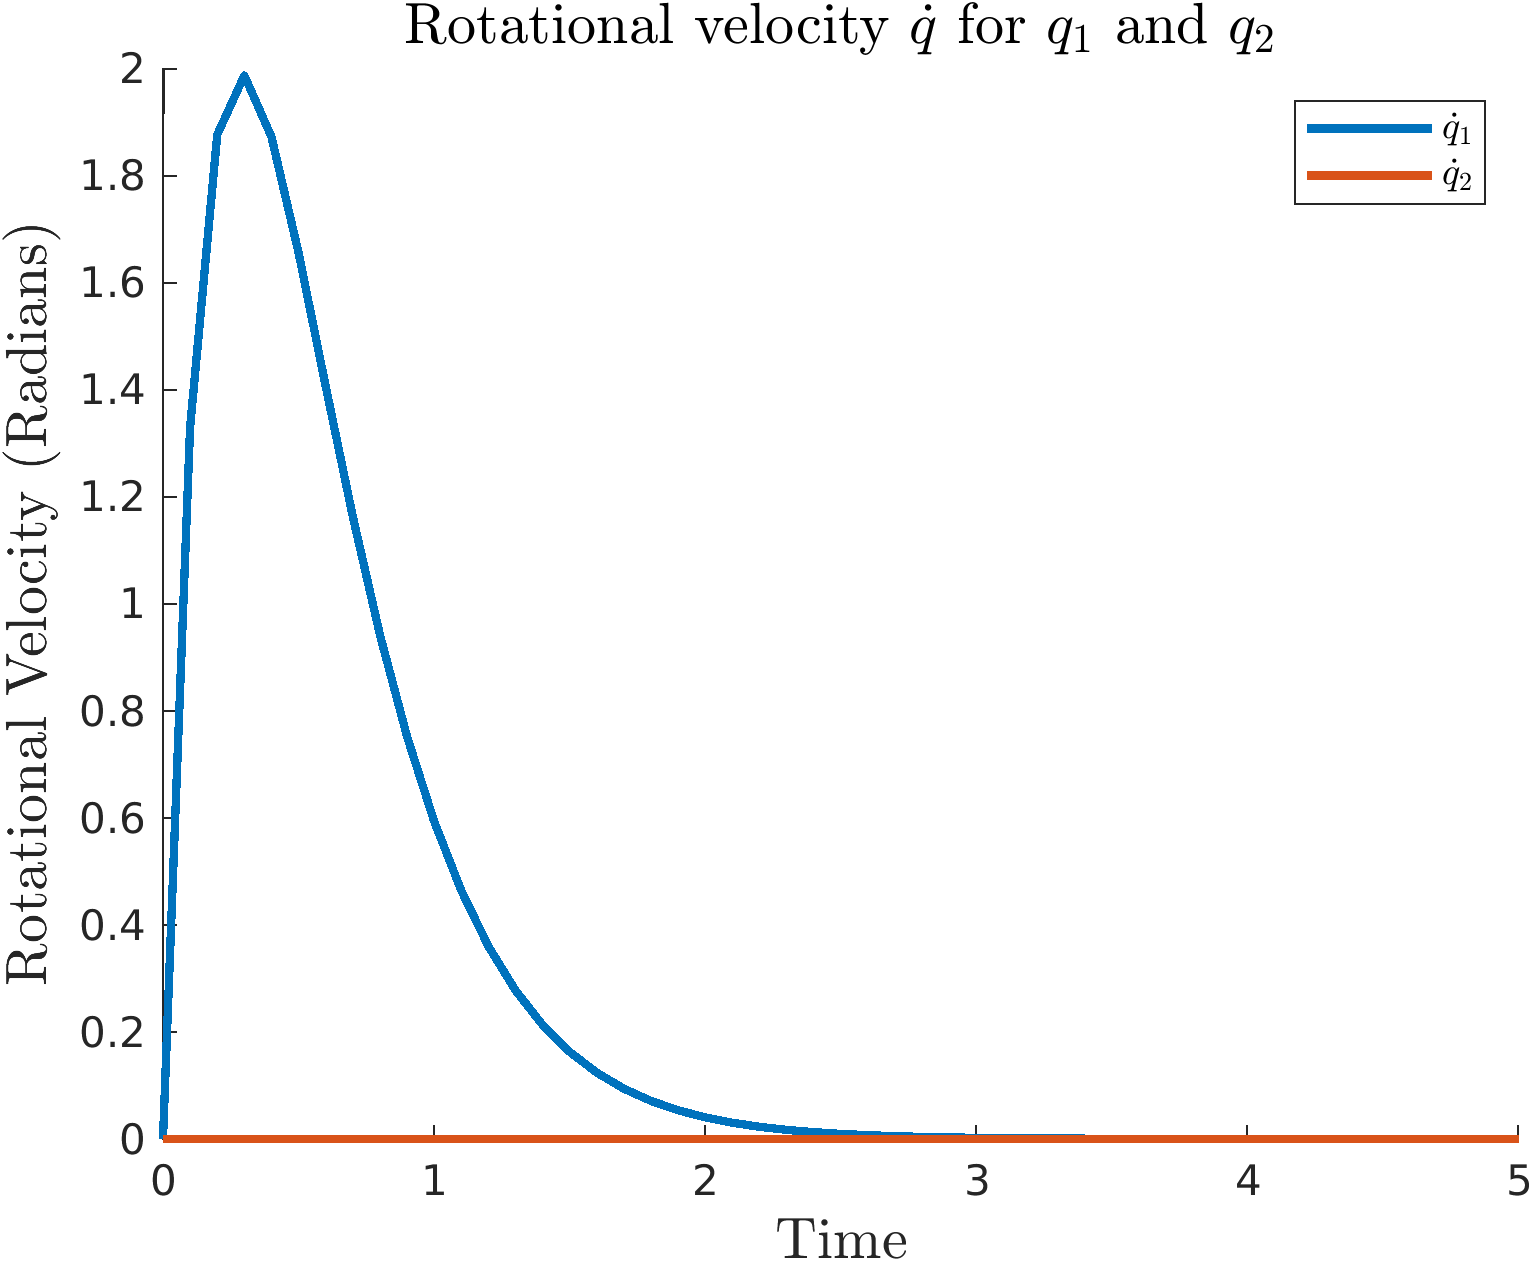
\includegraphics[width = \textwidth]{figures/rotational-velocity-c2.png}
        \caption{Rotational velocity over time}
    \end{subfigure}
    \caption{System response with $x_d=\begin{bmatrix} \frac{\pi}{2} & 0 & 0 & 0 \end{bmatrix}^T$}
    \label{fig:c-2_results}
\end{figure}


\subsection*{III: $x_d = \begin{bmatrix} \frac{\pi}{4} & \frac{\pi}{4} & 0 & 0 \end{bmatrix}^T$}

\begin{figure}[H]
    \centering
    \begin{subfigure}{0.325\textwidth}
        \centering
        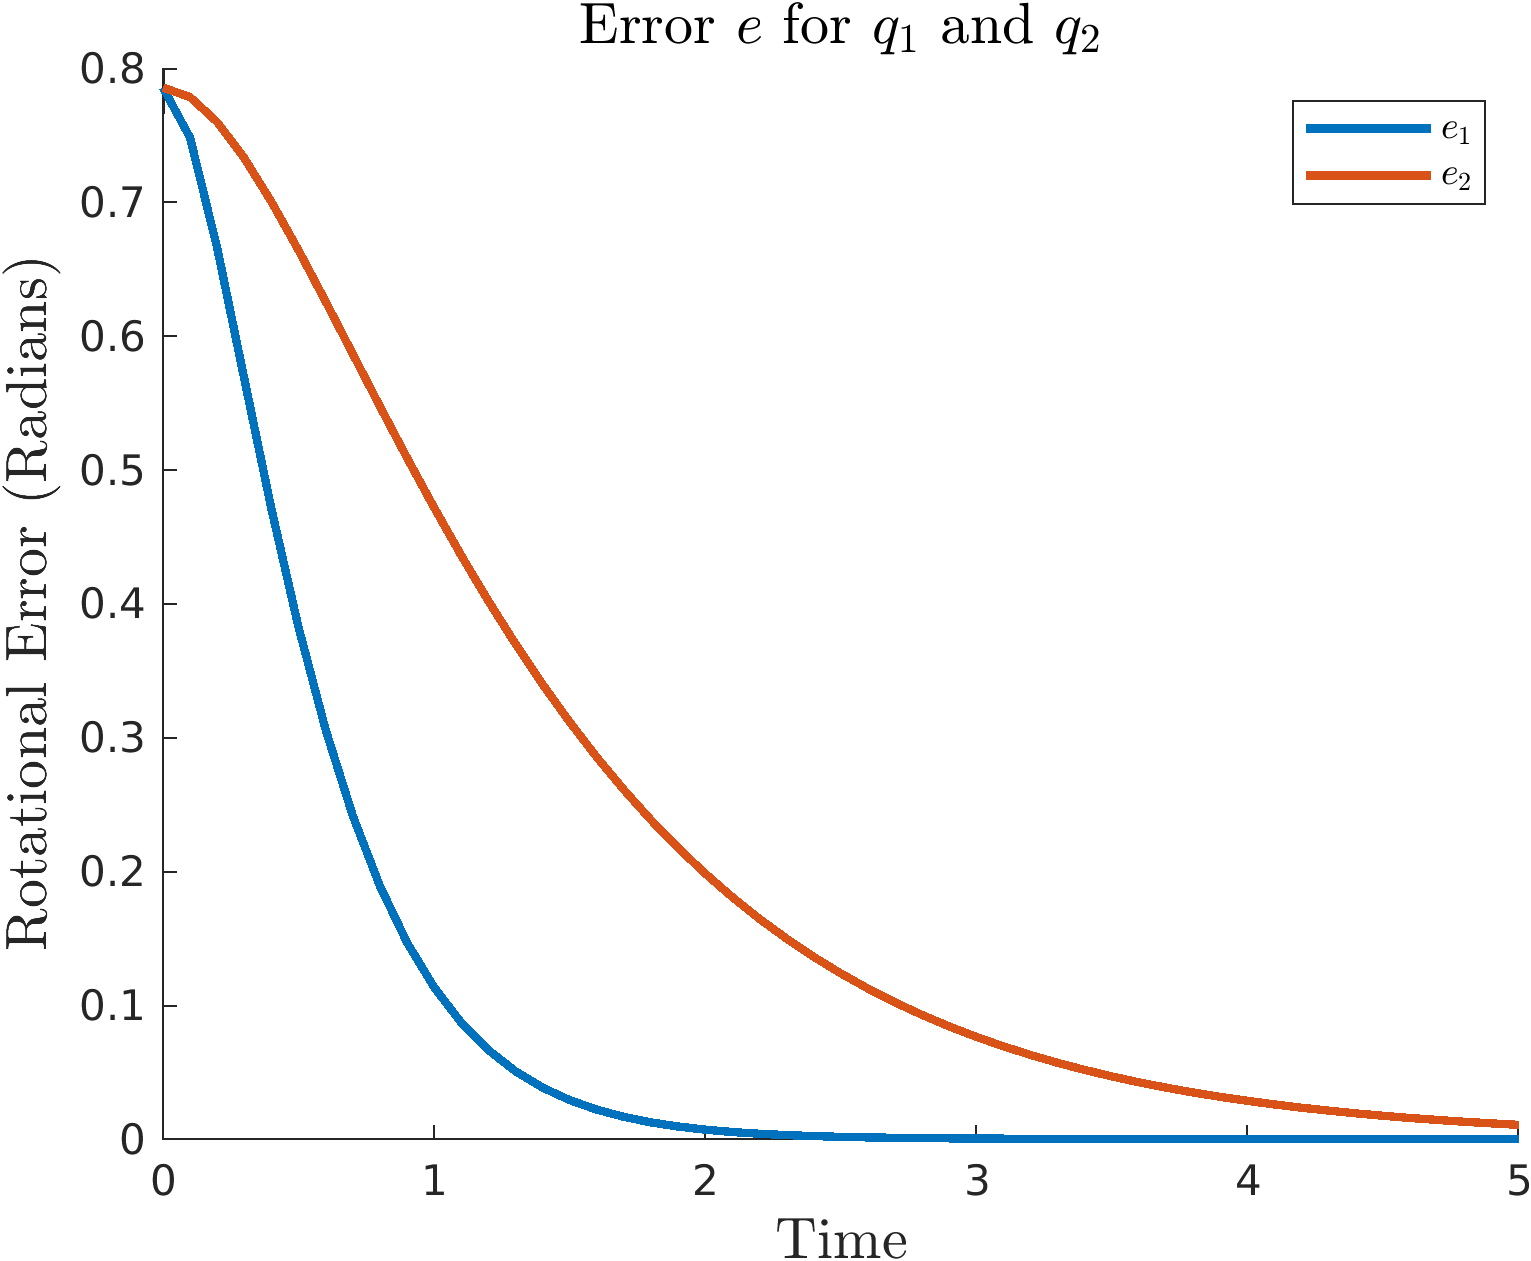
\includegraphics[width = \textwidth]{figures/error-c3.png}
        \caption{Error over time}
    \end{subfigure}
    \begin{subfigure}{0.325\textwidth}
        \centering
        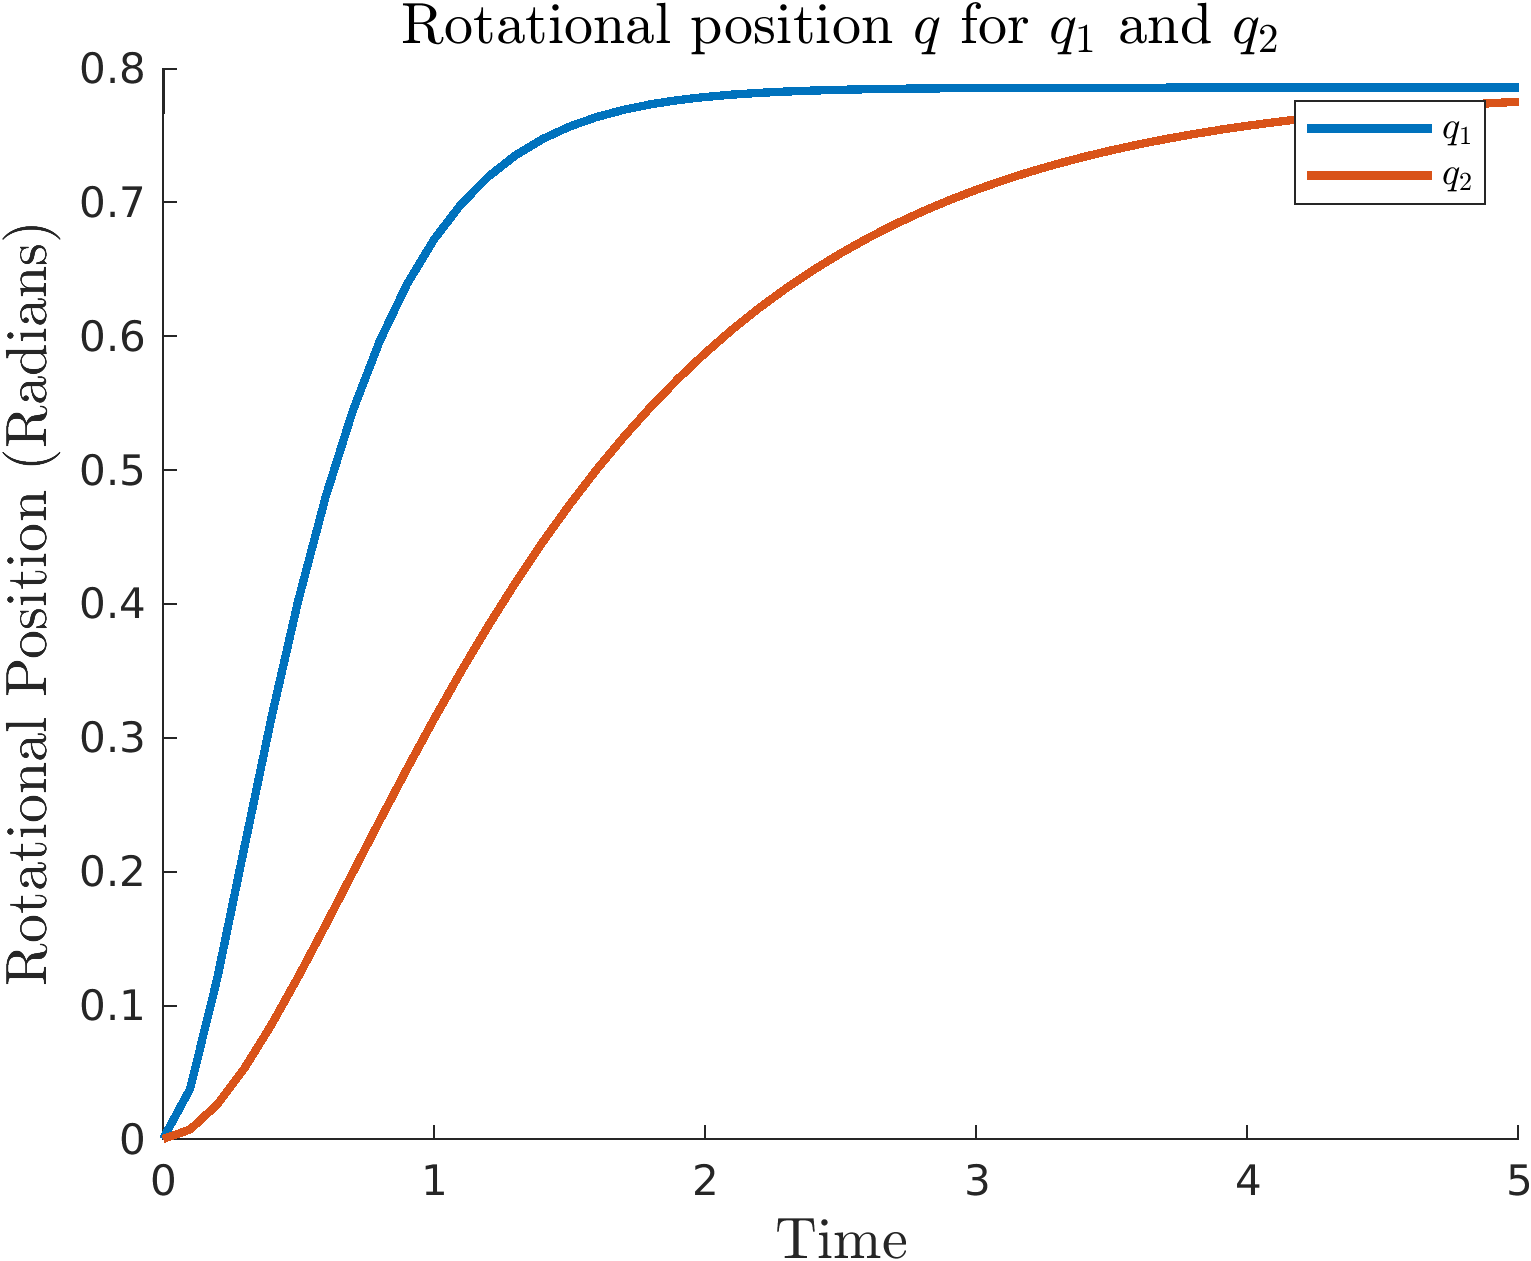
\includegraphics[width = \textwidth]{figures/rotational-position-c3.png}
        \caption{Rotational position over time}
    \end{subfigure}
    \begin{subfigure}{0.325\textwidth}
        \centering
        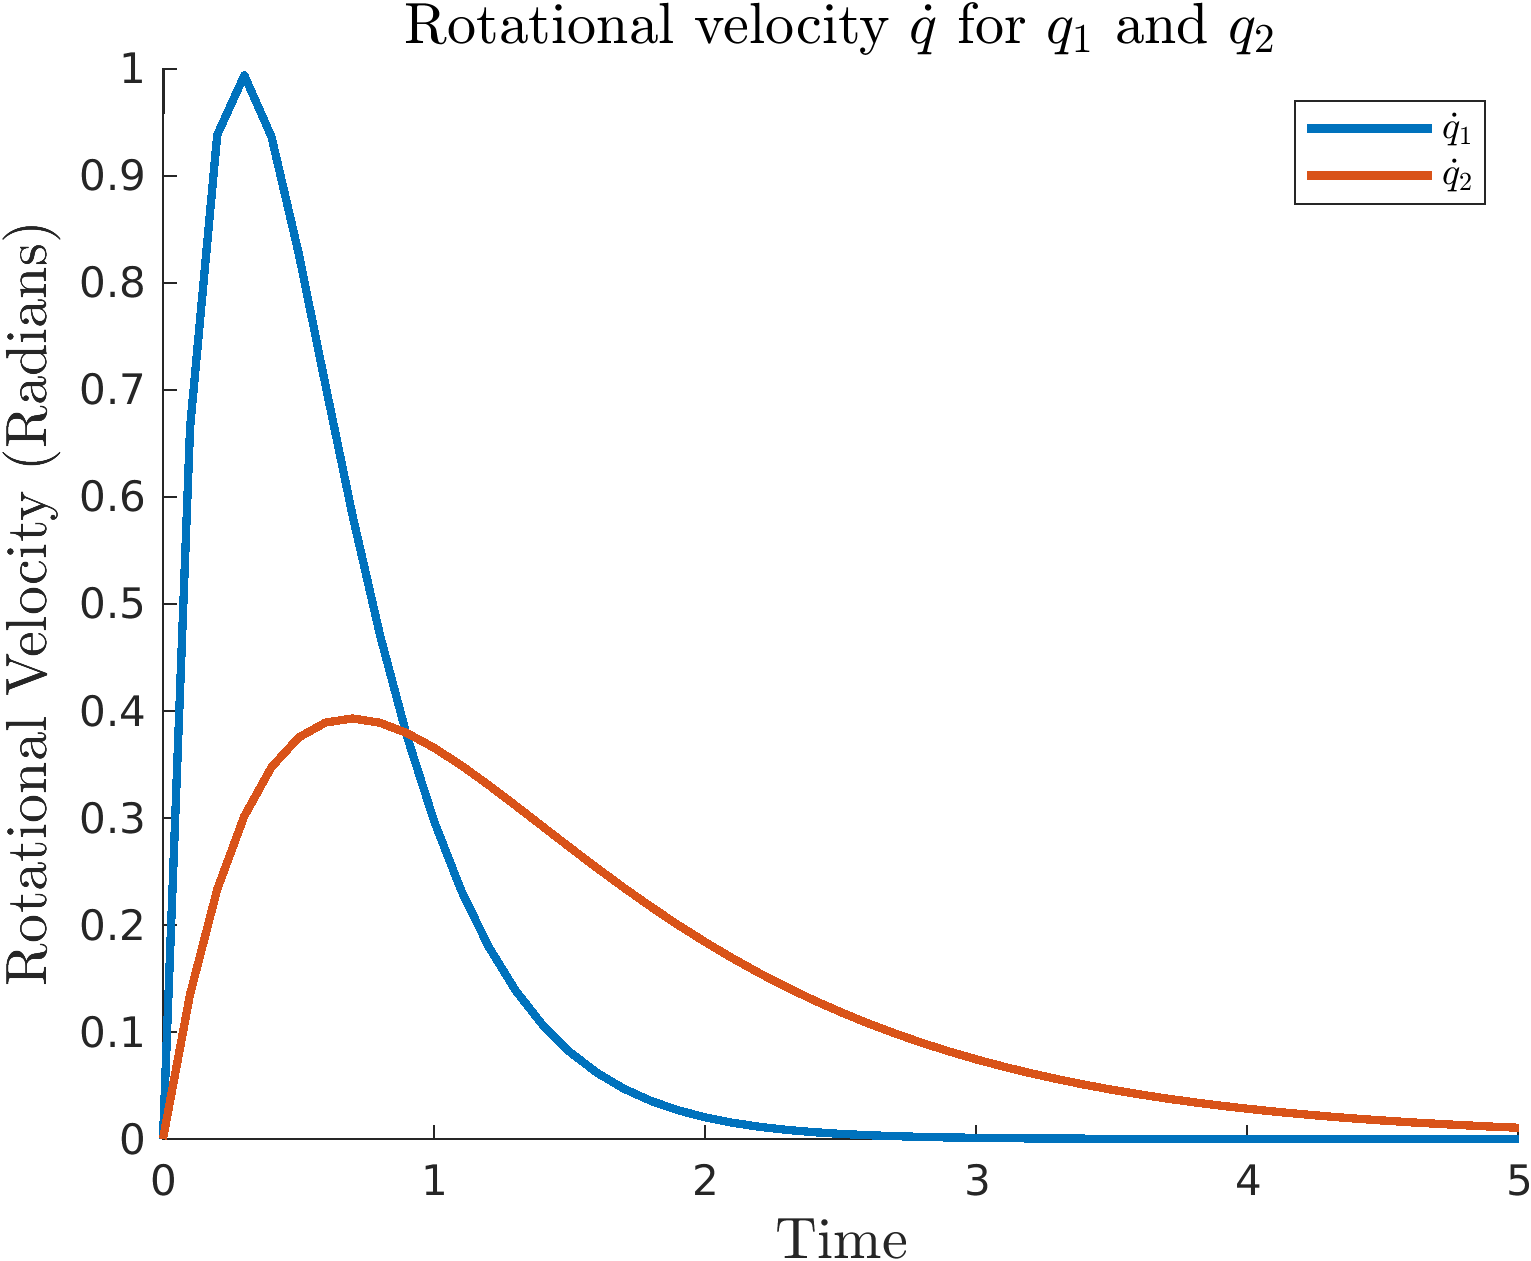
\includegraphics[width = \textwidth]{figures/rotational-velocity-c3.png}
        \caption{Rotational velocity over time}
    \end{subfigure}
    \caption{System response with $x_d=\begin{bmatrix} \frac{\pi}{4} & \frac{\pi}{4} & 0 & 0 \end{bmatrix}^T$}
    \label{fig:c-3_results}
\end{figure}

\section*{Part D}

In this section, we are considering how a limit of torque for each given motor would affect our system. To this point, we have operated under the assumption that our system either has no upper limit in torque, or a sufficiently large capability such that we will not approach its limit. This is not accurate towards a real-life case. Motors have maximum torques that we can provide, thus saturating the response of our system.

To investigate, we are looking at a several limits, such that $u_{limit} = \{ 500, 200, 75 \}$. We will limit the torque output of our system by utilizing a function $u_{bound}$, where:

\begin{equation}
    u_{bound} = min( max(u(e), -u_{limit}), u_{limit})
\end{equation}

...essentially - calculate our resultant $u(e)$ for the given state, but bound it to $\pm u_{limit}$. We will be utilizing $x_d=\begin{bmatrix} \frac{\pi}{4} & \frac{\pi}{4} & 0 & 0 \end{bmatrix}^T$ so as to see movement of both joints and compare it to our unsaturated results in part C-III.

\subsection*{I - $u_{limit} = 500$}

\begin{figure}[H]
    \centering
    \begin{subfigure}{0.325\textwidth}
        \centering
        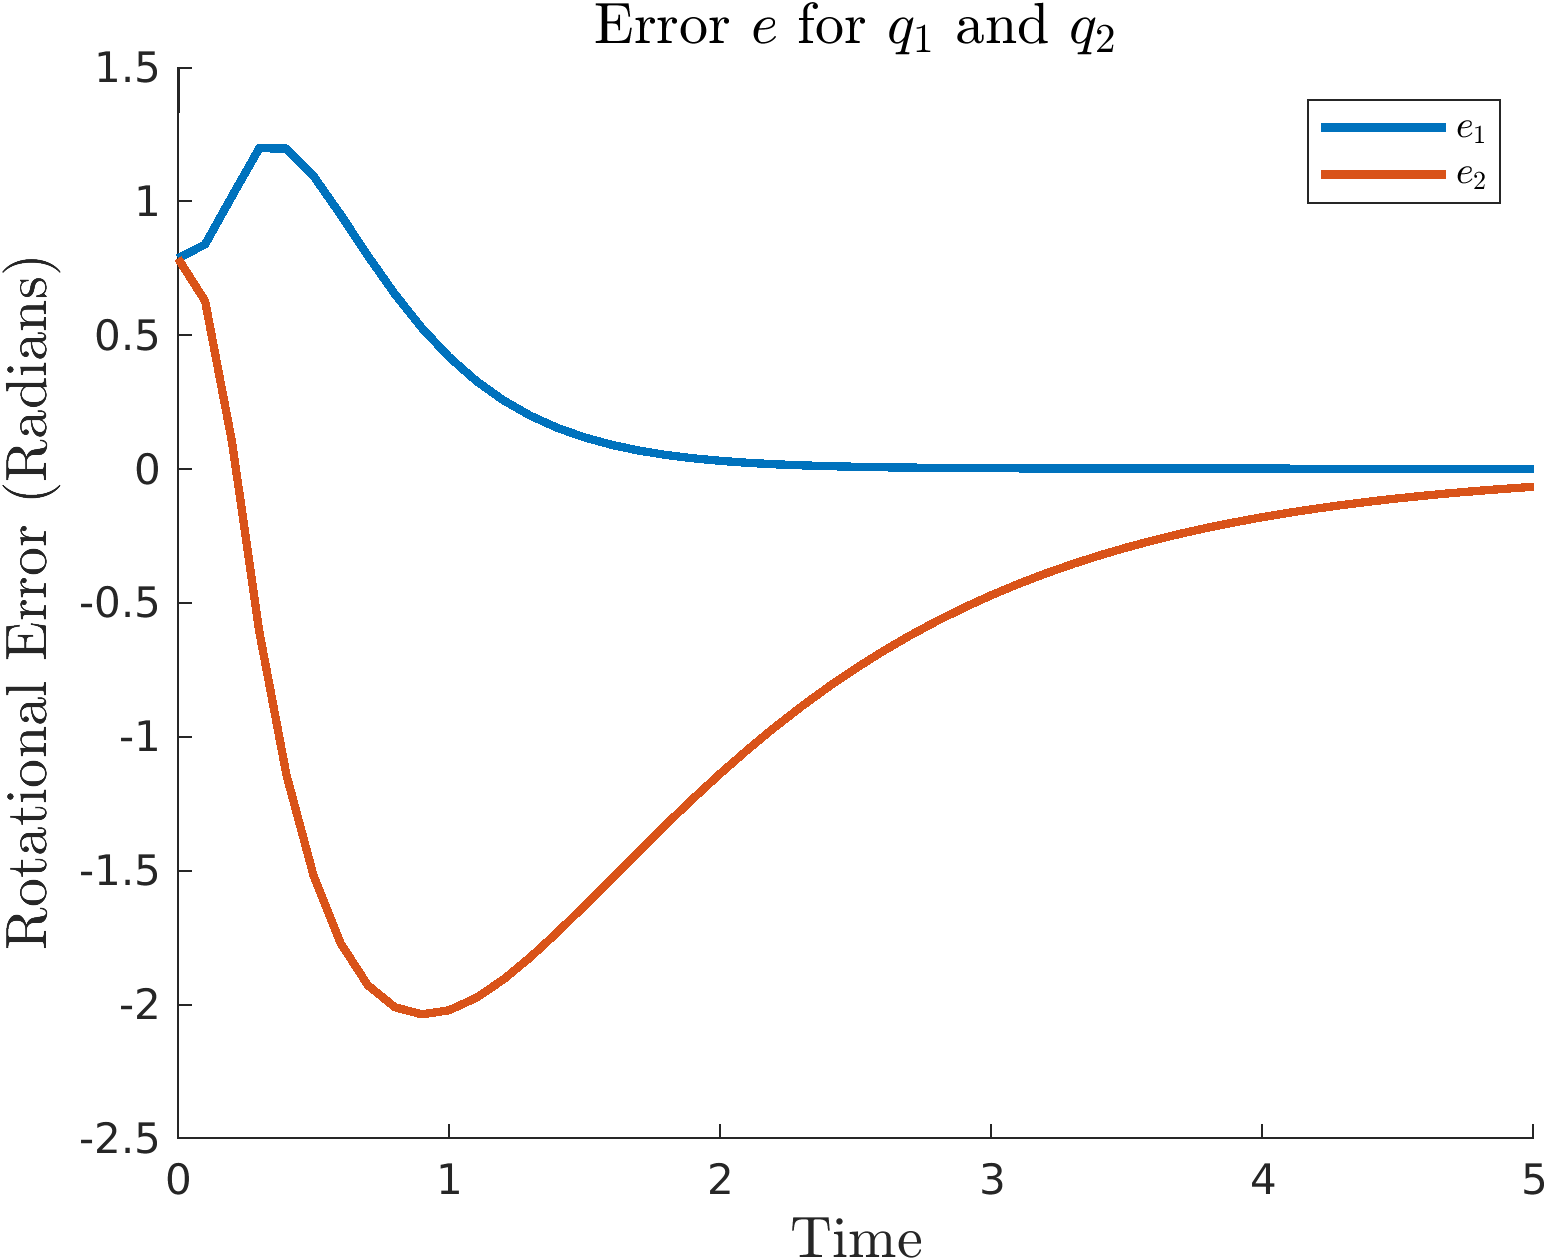
\includegraphics[width = \textwidth]{figures/error-d1.png}
        \caption{Error over time}
    \end{subfigure}
    \begin{subfigure}{0.325\textwidth}
        \centering
        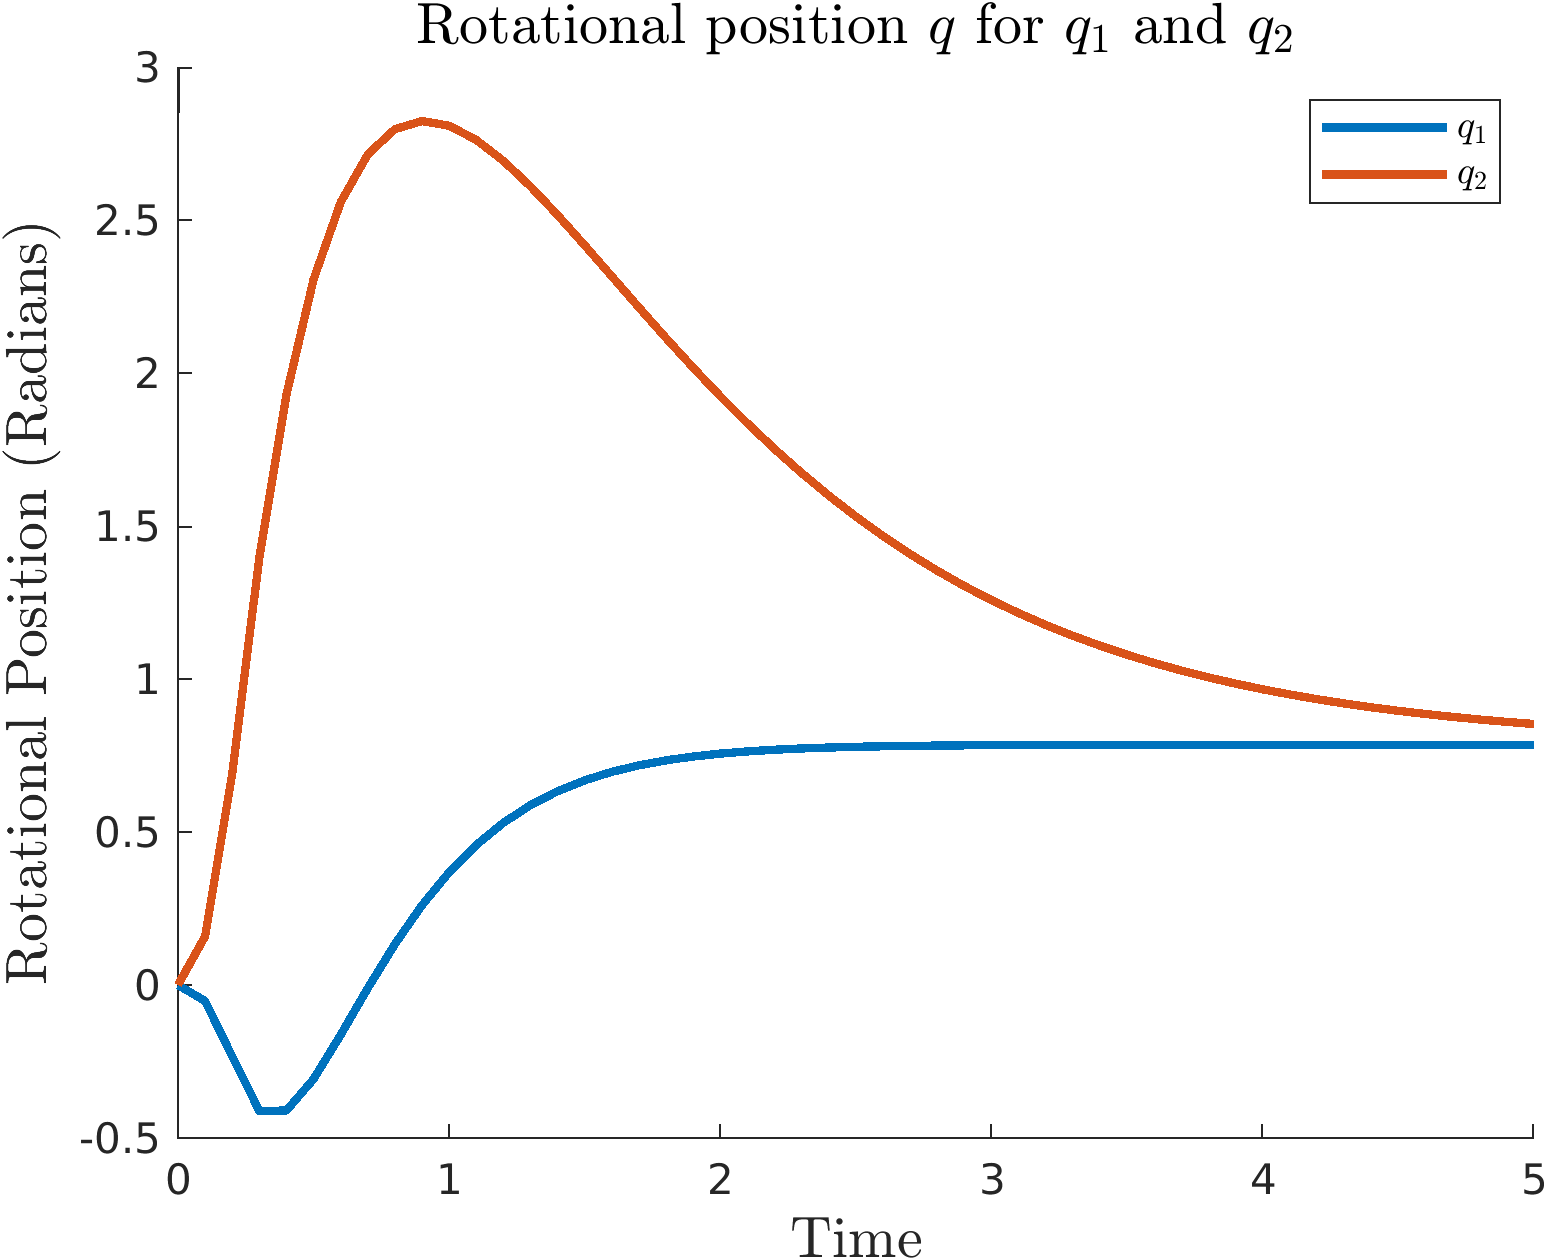
\includegraphics[width = \textwidth]{figures/rotational-position-d1.png}
        \caption{Rotational position over time}
    \end{subfigure}
    \begin{subfigure}{0.325\textwidth}
        \centering
        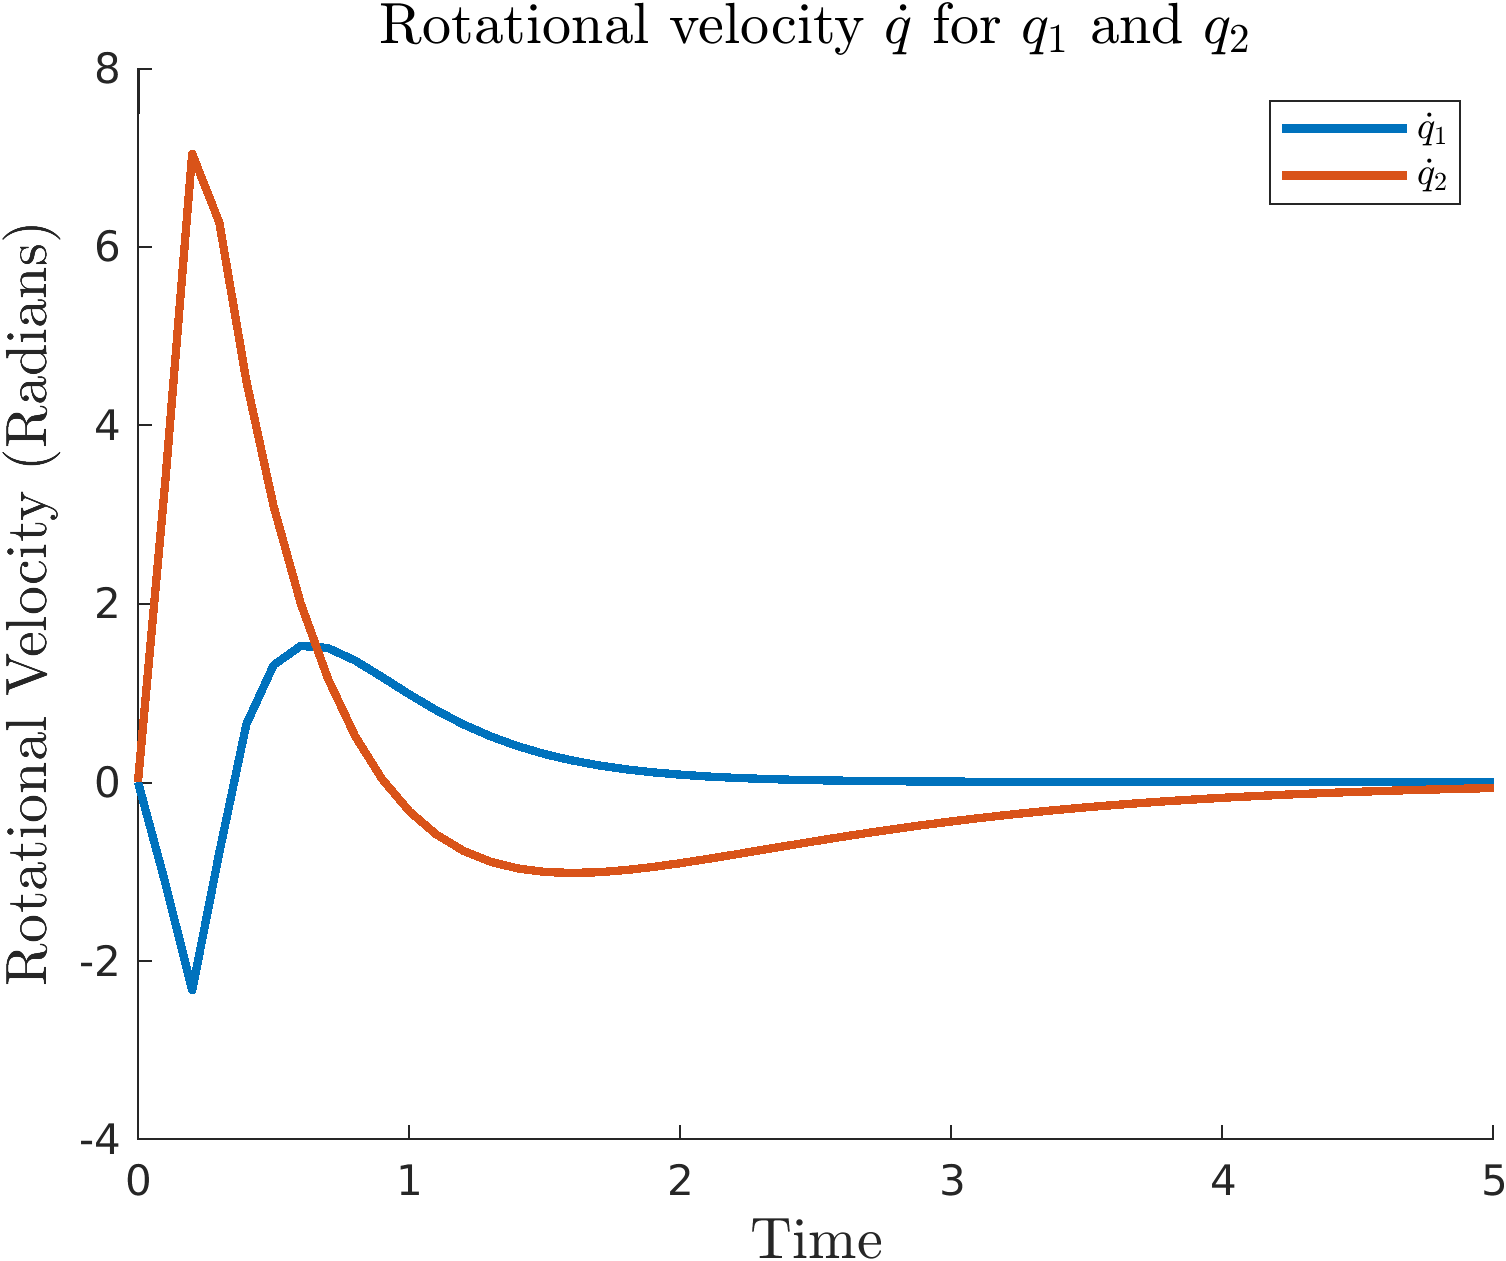
\includegraphics[width = \textwidth]{figures/rotational-velocity-d1.png}
        \caption{Rotational velocity over time}
    \end{subfigure}
    \caption{System response with $x_d=\begin{bmatrix} \frac{\pi}{4} & \frac{\pi}{4} & 0 & 0 \end{bmatrix}^T$ and $u_{limit} = 500$}
    \label{fig:d-1_results}
\end{figure}

Here we see the system take a much larger error caused by an inability to handle the resulting torque require for both arms moving into position. We see similar changes in the velocities and the accelerations for the arms, where the arm has a period of time where it can not handle the required torque to move the arm into position.

\subsection*{II - $u_{limit} = 200$}

\begin{figure}[H]
    \centering
    \begin{subfigure}{0.325\textwidth}
        \centering
        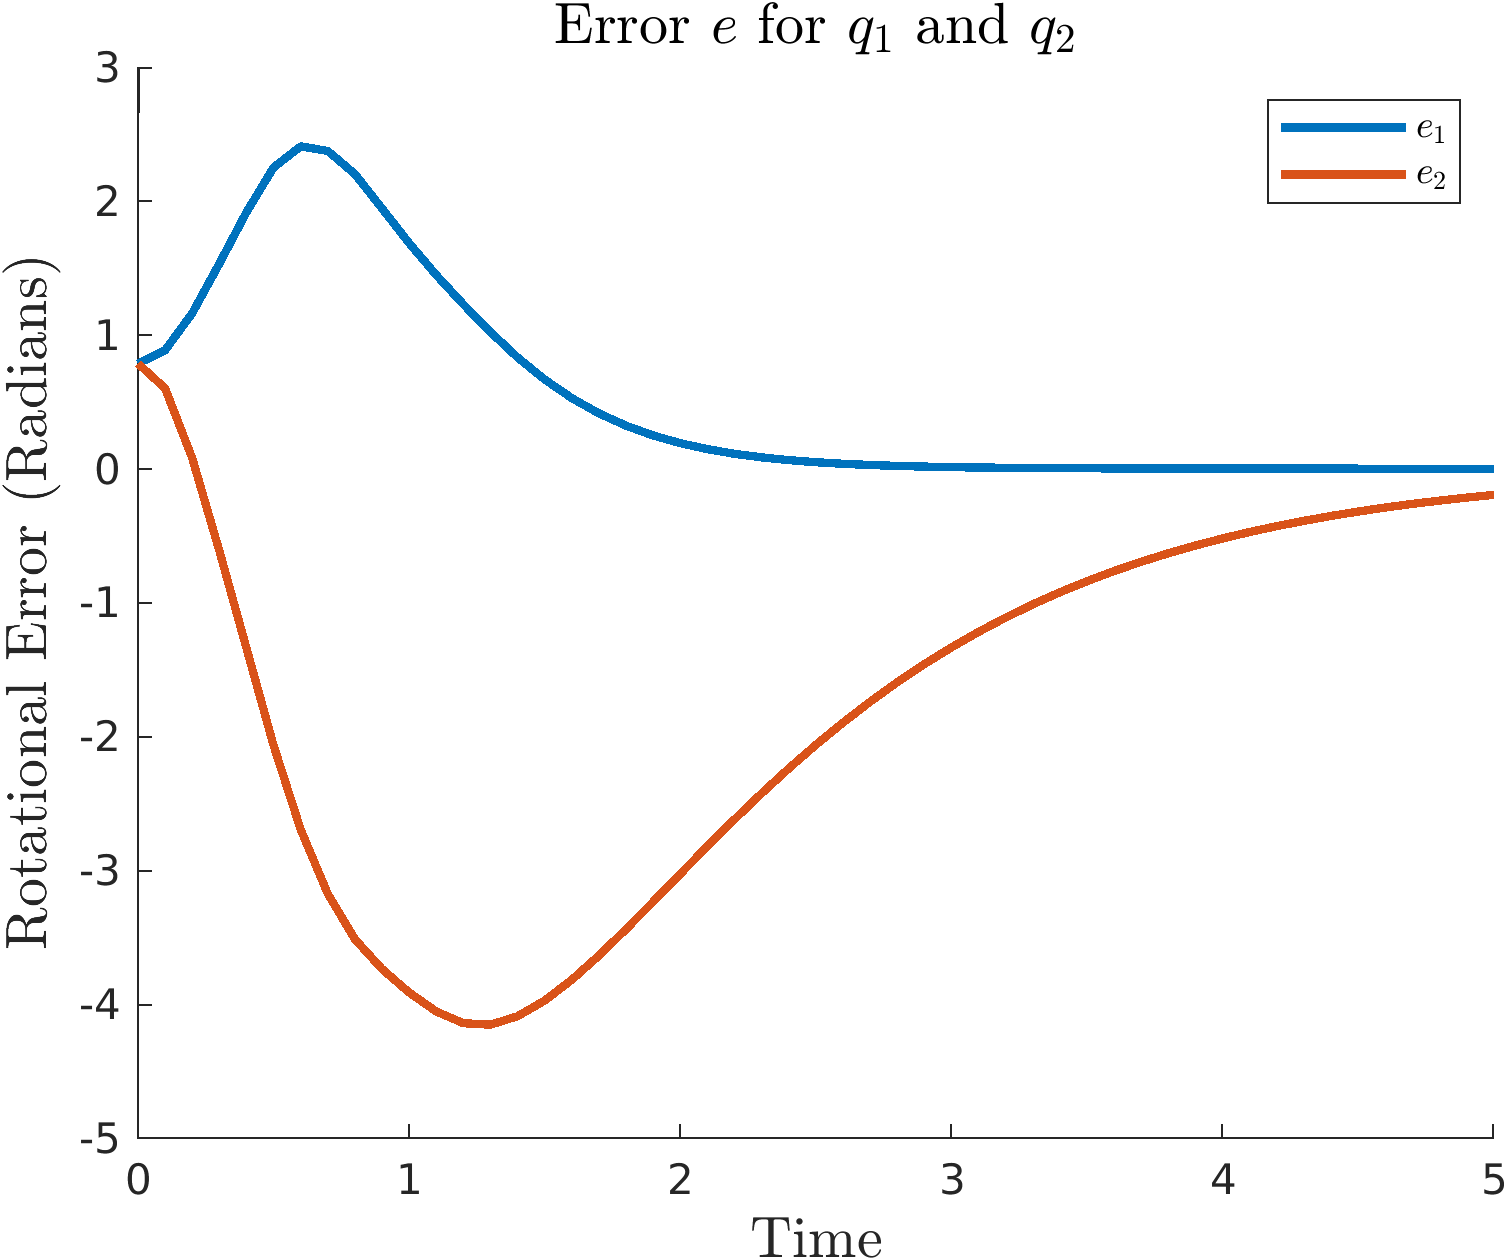
\includegraphics[width = \textwidth]{figures/error-d2.png}
        \caption{Error over time}
    \end{subfigure}
    \begin{subfigure}{0.325\textwidth}
        \centering
        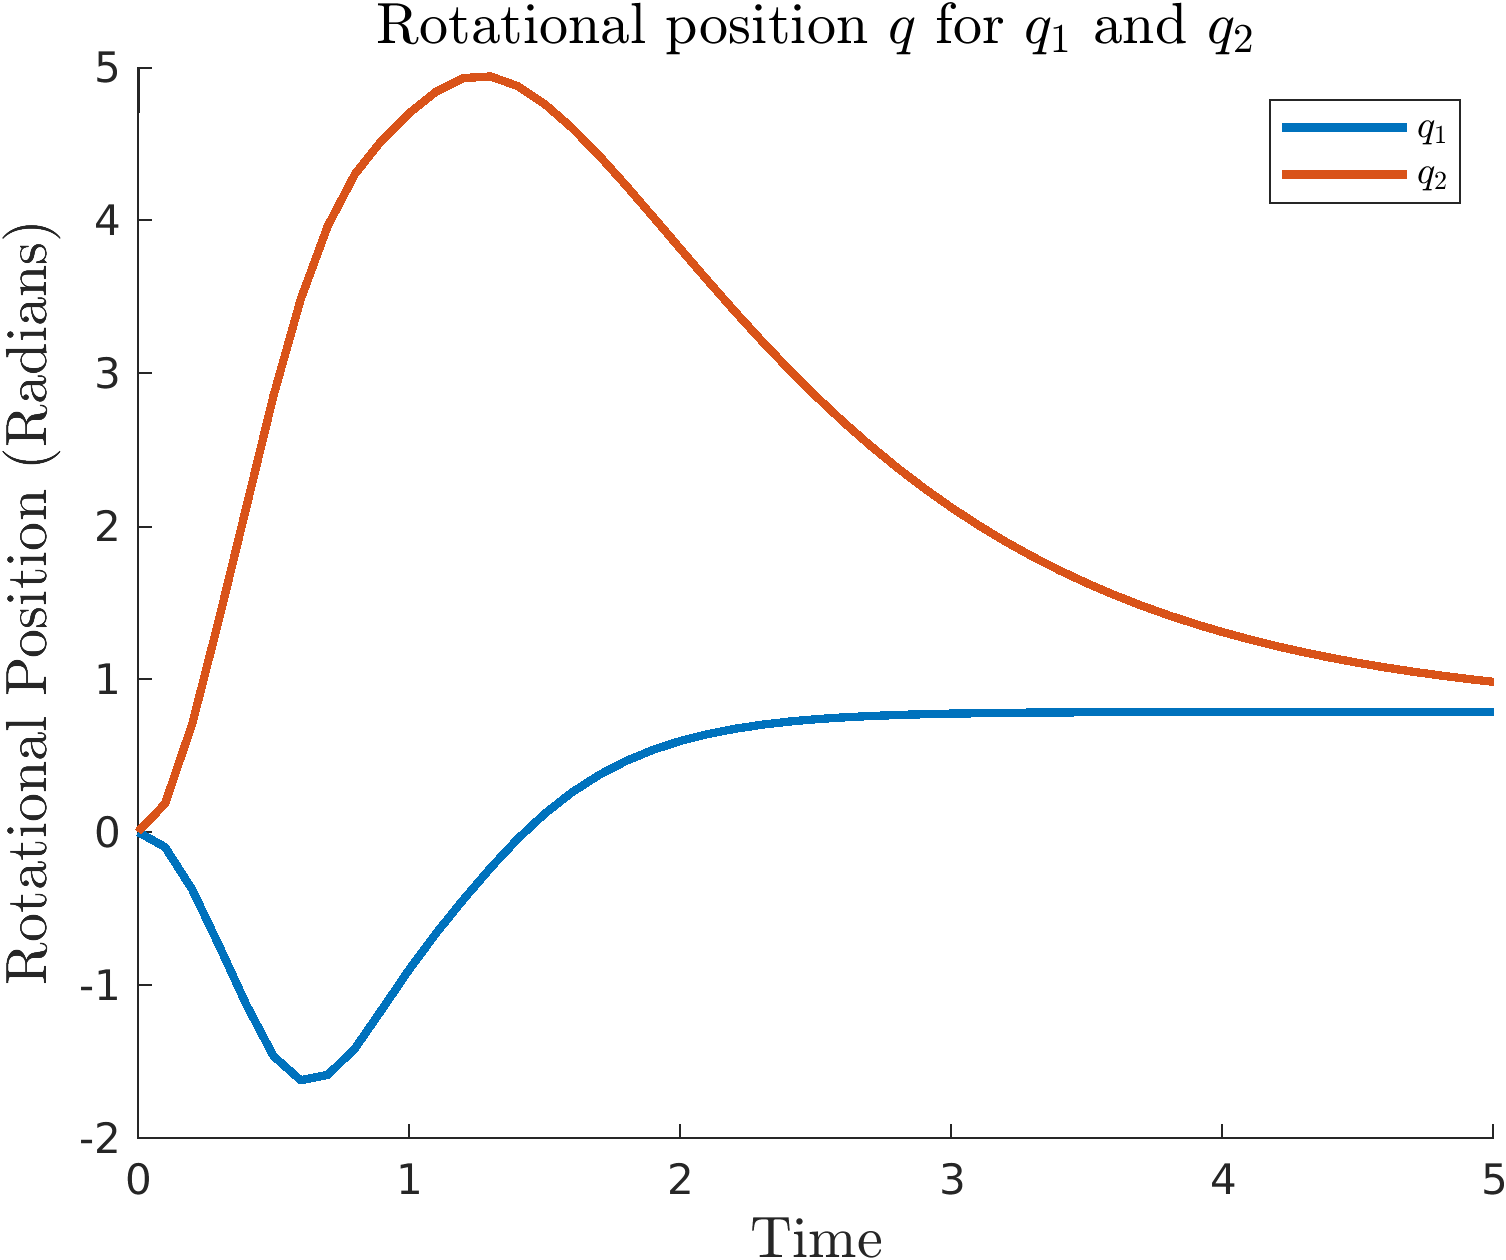
\includegraphics[width = \textwidth]{figures/rotational-position-d2.png}
        \caption{Rotational position over time}
    \end{subfigure}
    \begin{subfigure}{0.325\textwidth}
        \centering
        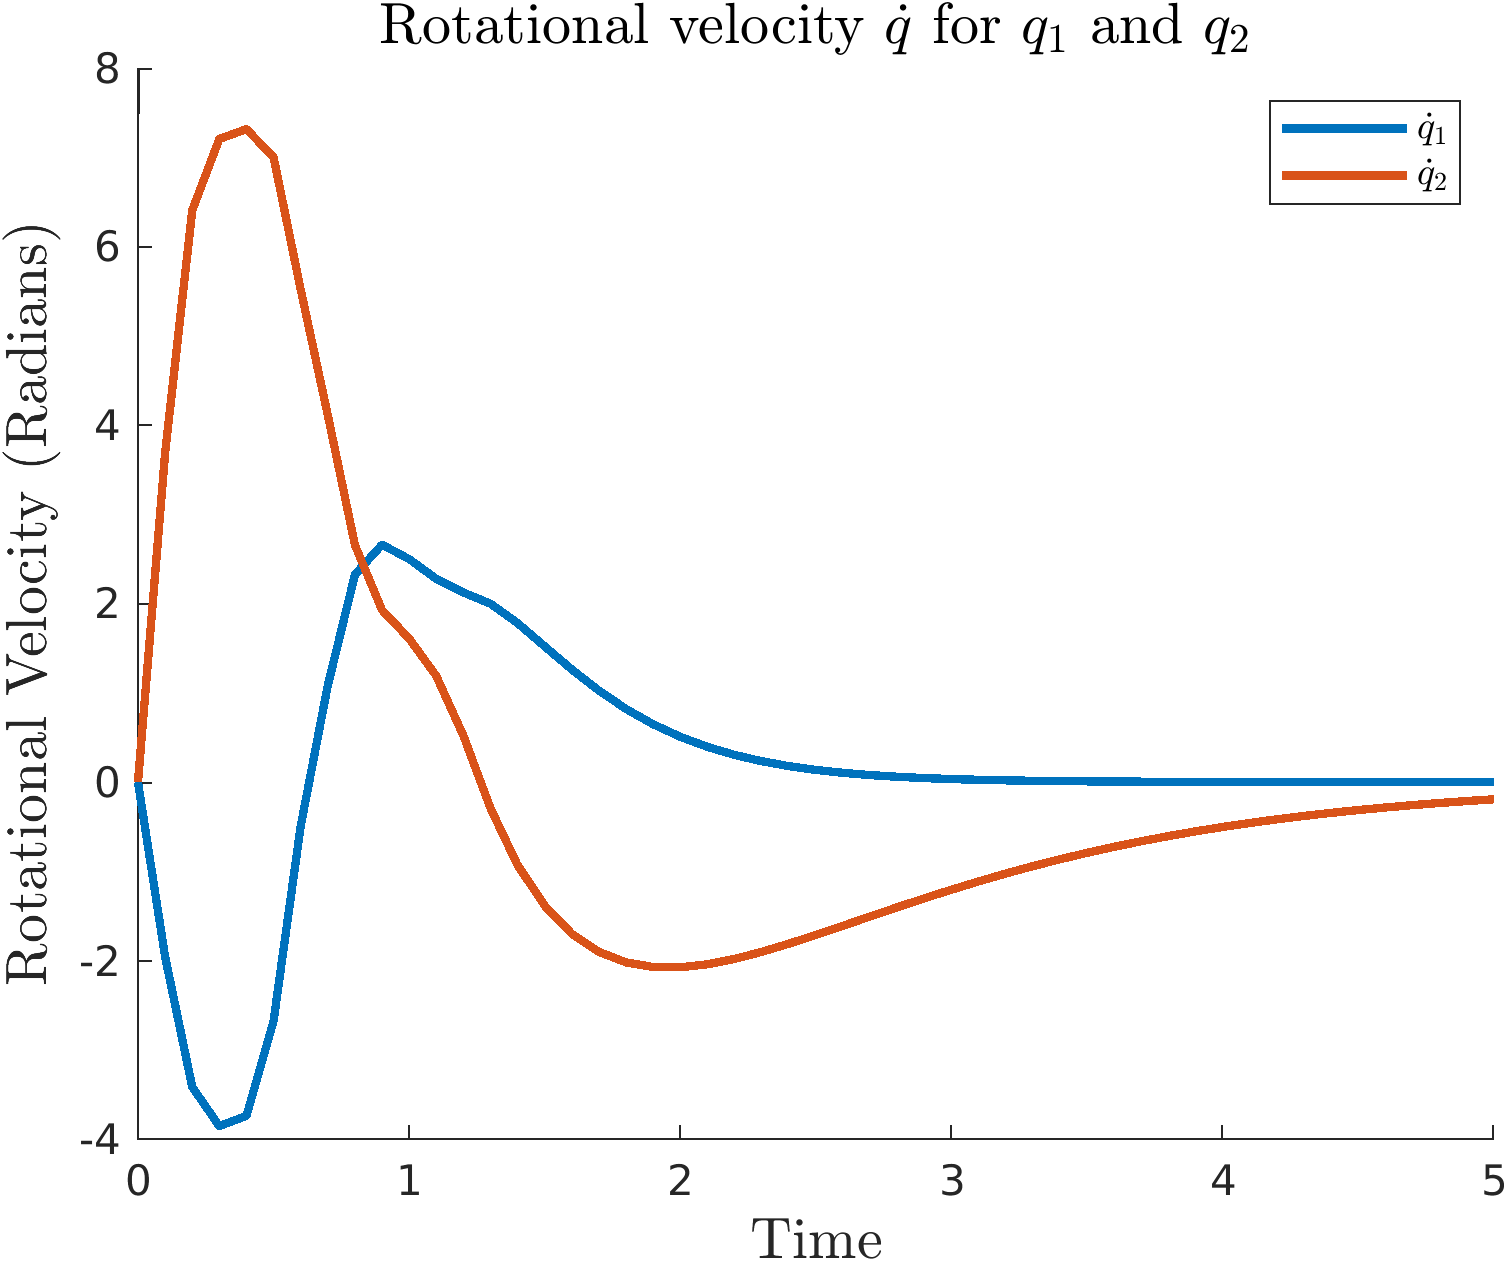
\includegraphics[width = \textwidth]{figures/rotational-velocity-d2.png}
        \caption{Rotational velocity over time}
    \end{subfigure}
    \caption{System response with $x_d=\begin{bmatrix} \frac{\pi}{4} & \frac{\pi}{4} & 0 & 0 \end{bmatrix}^T$ and $u_{limit} = 200$}
    \label{fig:d-2_results}
\end{figure}

When utilize a much weaker motor, we begin to see the error $e_2$ begin to drastically increase. The system does still recover, causing the system to converge to its desired position just outside our time window of $5$ seconds. Velocities of the arm falling away from the desired position due to the limitation on torque rapidly rises. While our arm can reach its desired position, it is clear that the arm is struggling.

\subsection*{III - $u_{limit} = 75$}

\begin{figure}[H]
    \centering
    \begin{subfigure}{0.325\textwidth}
        \centering
        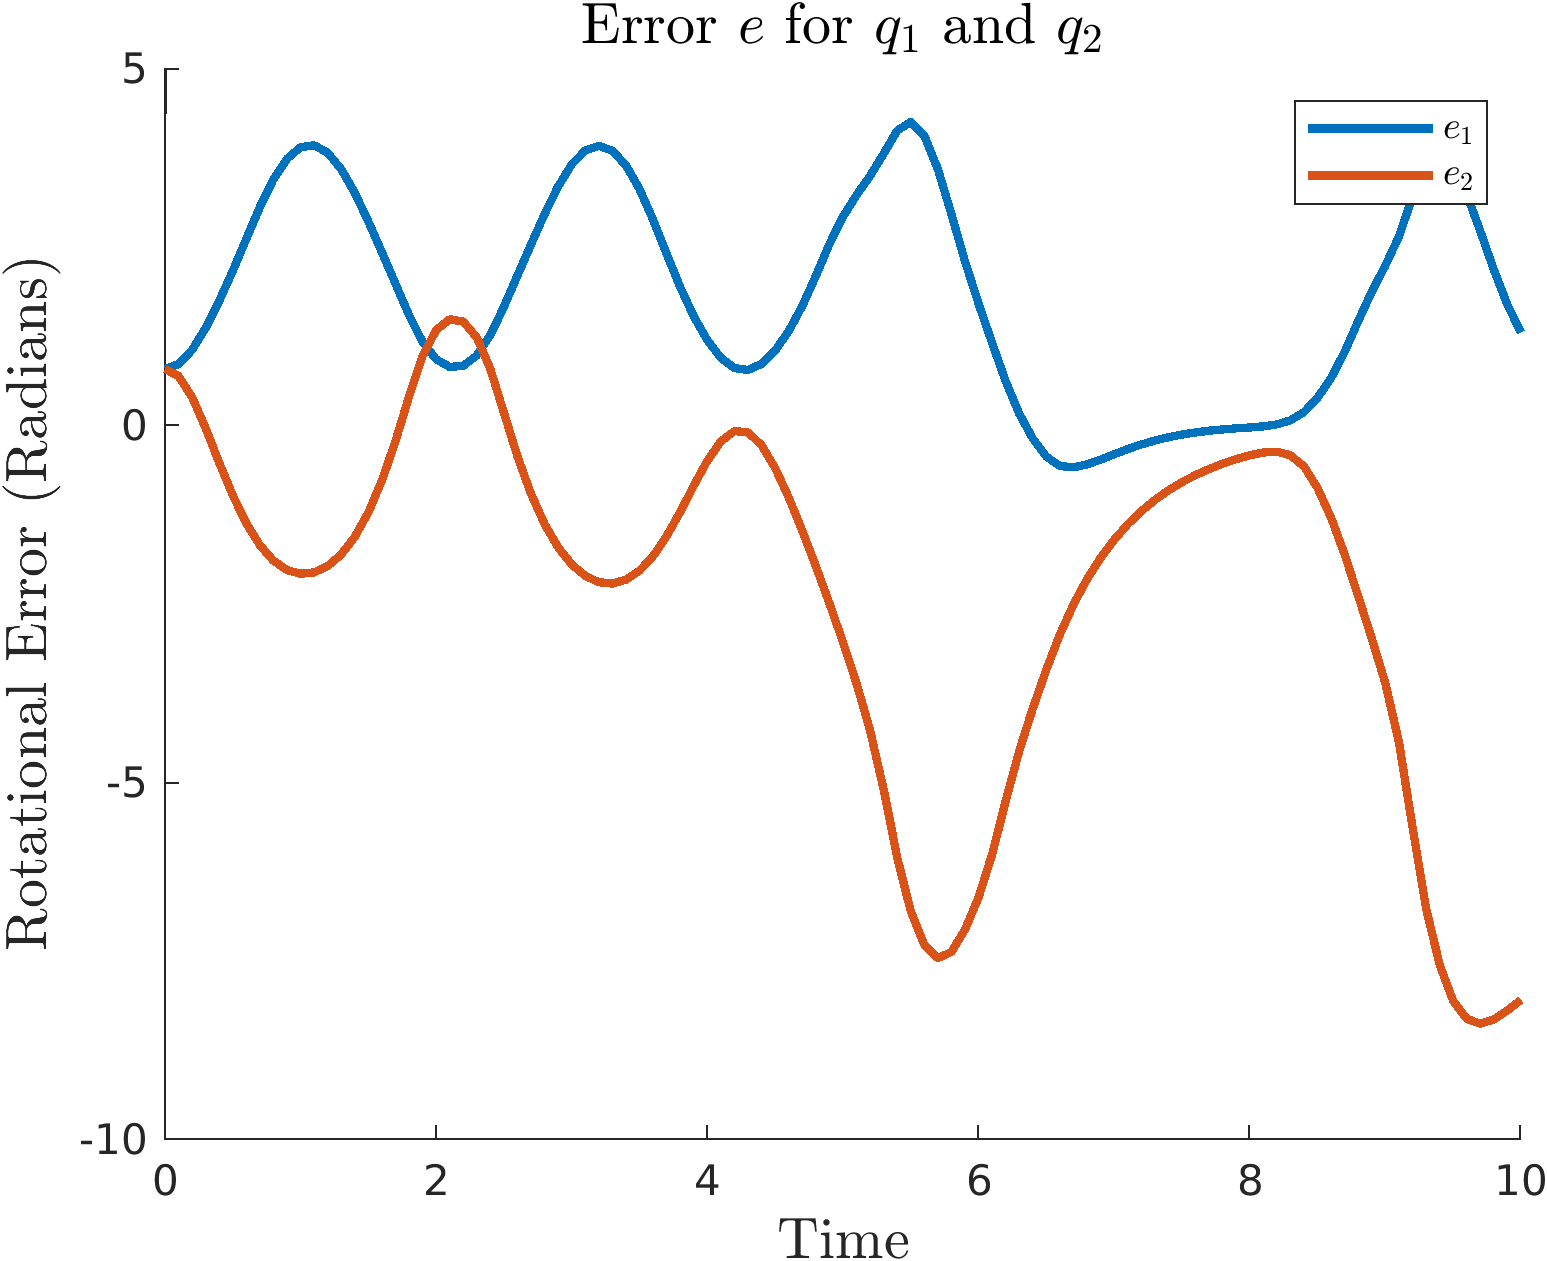
\includegraphics[width = \textwidth]{figures/error-d3.png}
        \caption{Error over time}
    \end{subfigure}
    \begin{subfigure}{0.325\textwidth}
        \centering
        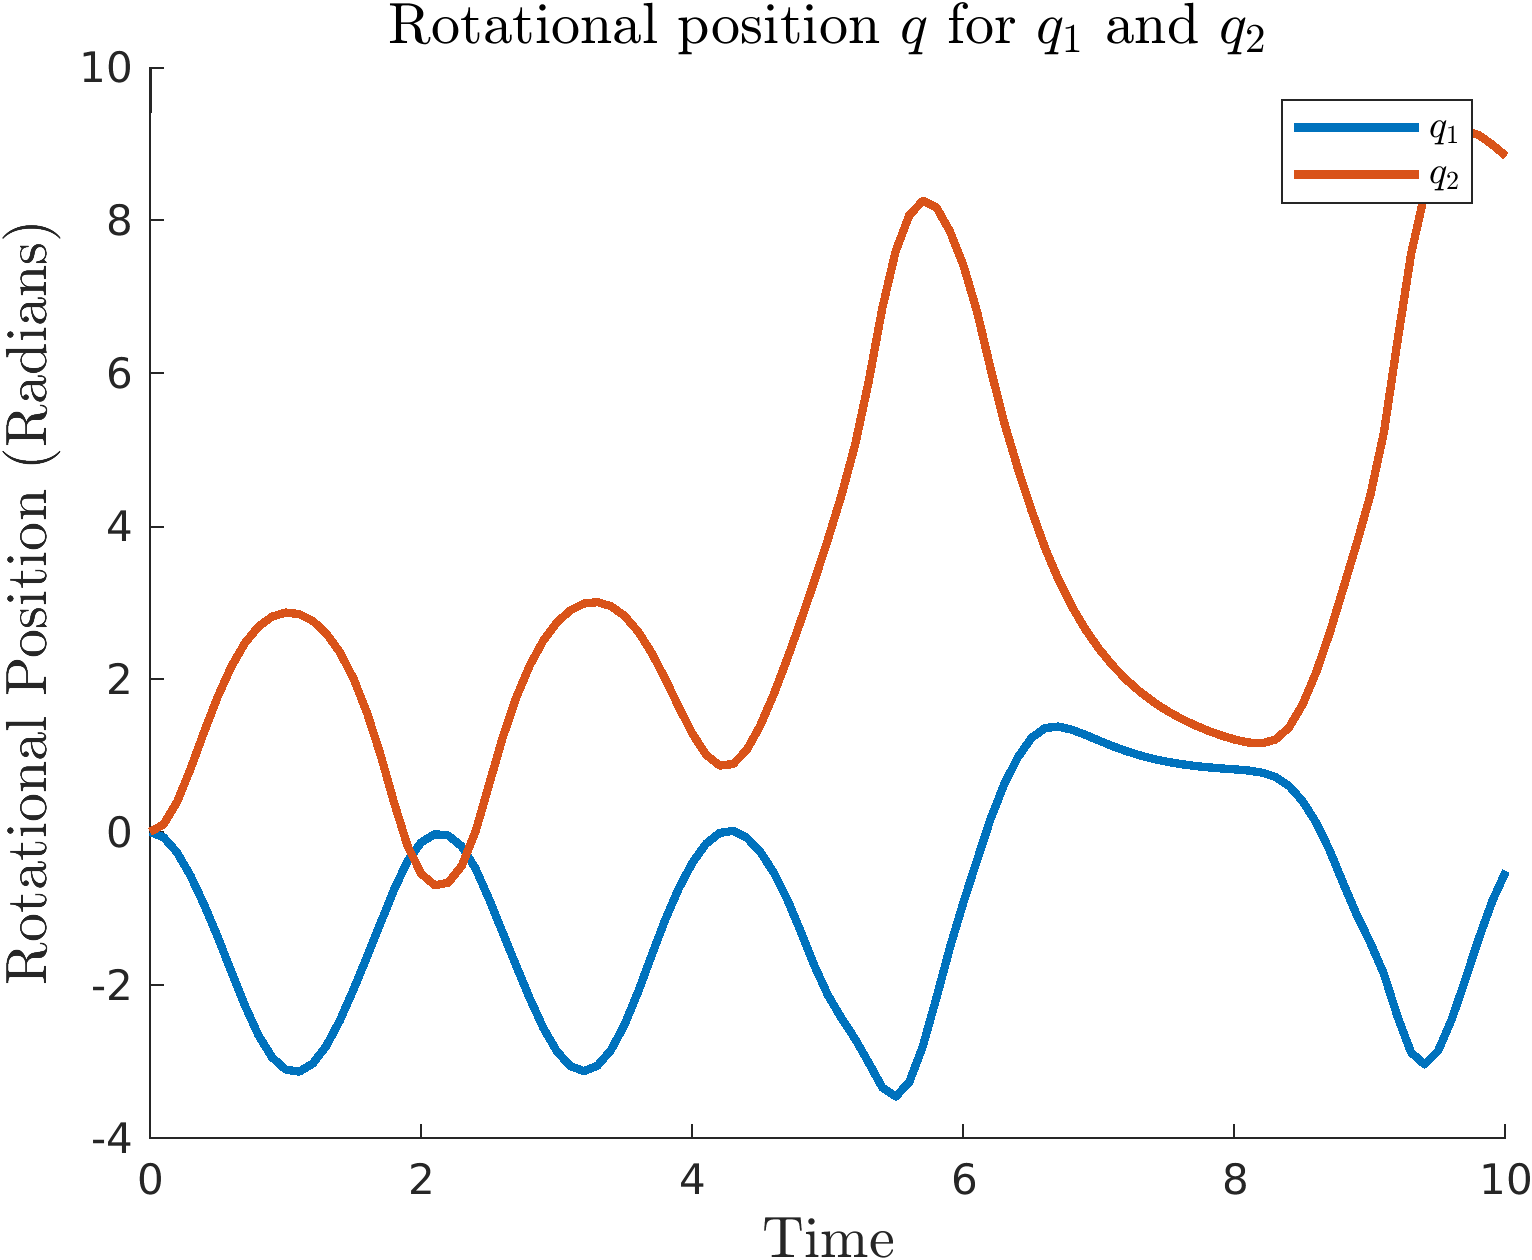
\includegraphics[width = \textwidth]{figures/rotational-position-d3.png}
        \caption{Rotational position over time}
    \end{subfigure}
    \begin{subfigure}{0.325\textwidth}
        \centering
        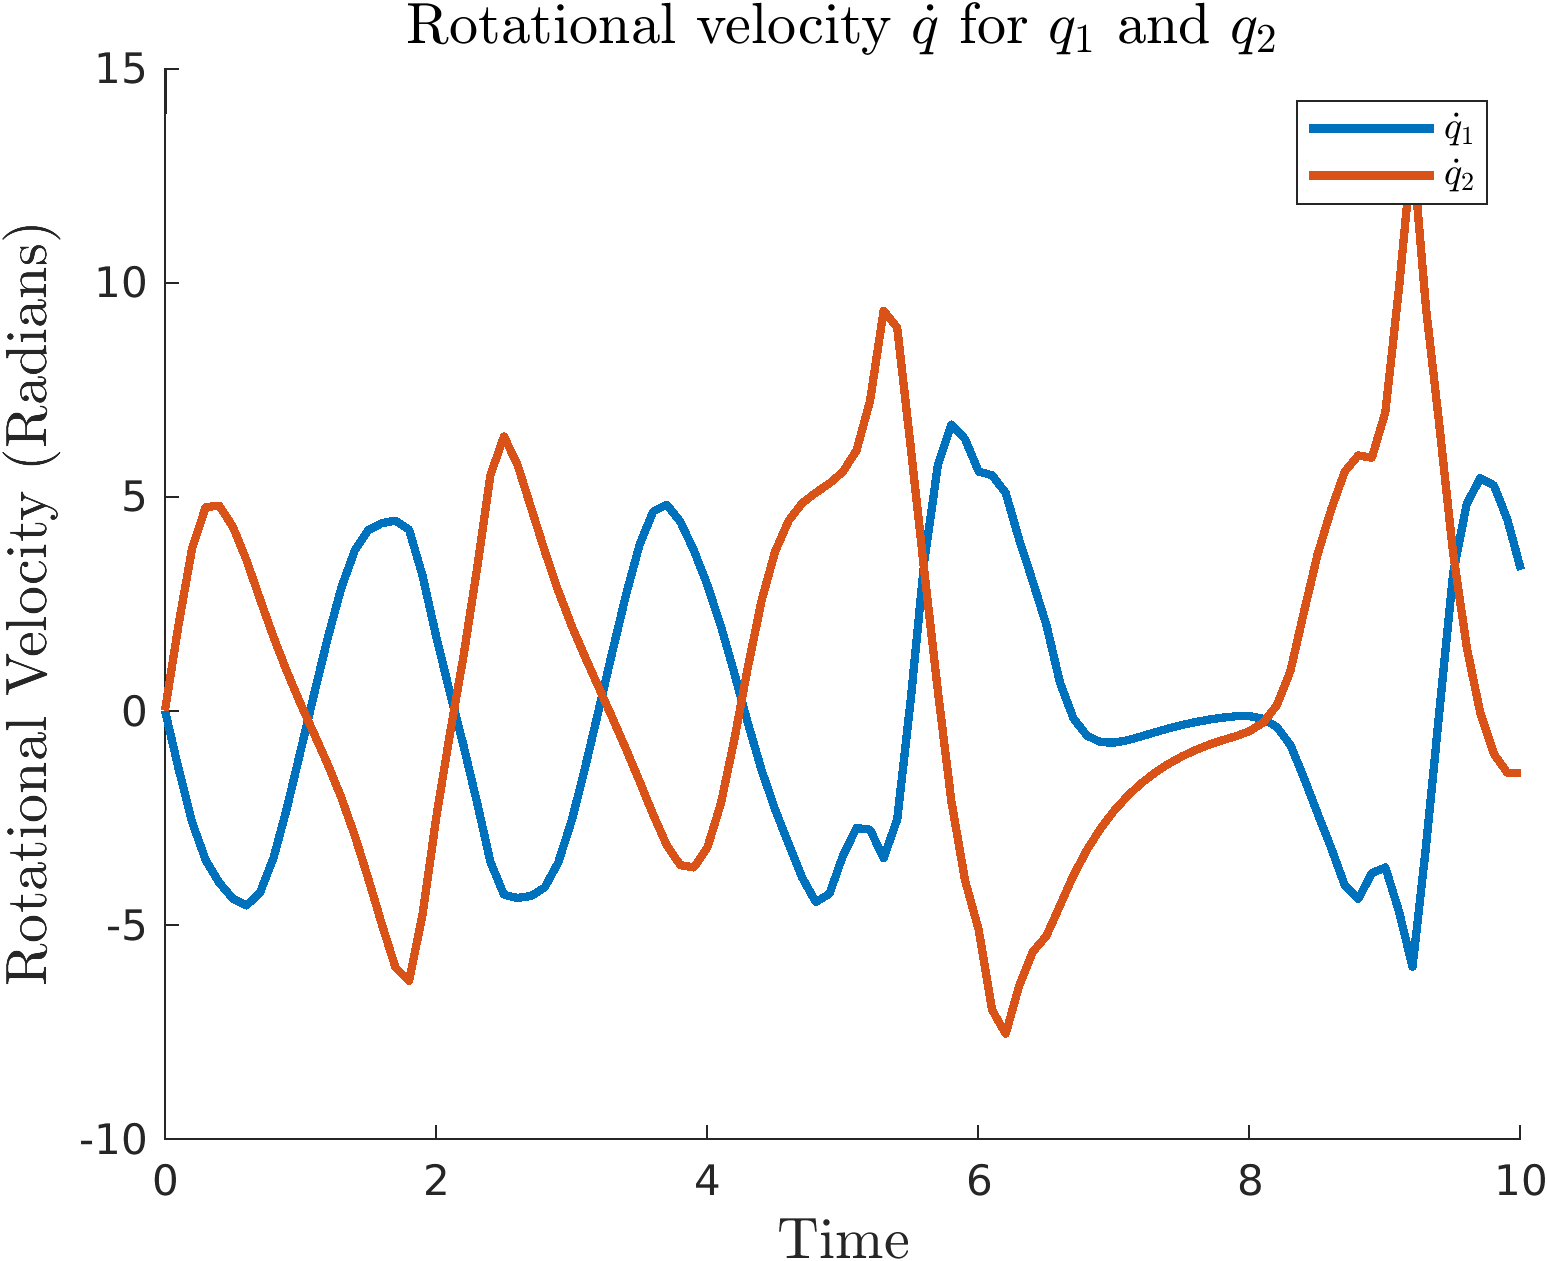
\includegraphics[width = \textwidth]{figures/rotational-velocity-d3.png}
        \caption{Rotational velocity over time}
    \end{subfigure}
    \caption{System response with $x_d=\begin{bmatrix} \frac{\pi}{4} & \frac{\pi}{4} & 0 & 0 \end{bmatrix}^T$ and $u_{limit} = 500$}
    \label{fig:d-3_results}
\end{figure}

Here we have limited our arm's joint motor torques too much. The arm cannot reach our desired position, even with a greatly exanded timespan of $10$ seconds. We see the arm wildly swinging with sharp accelerations due to the arm being unable to hold the arm stably in several of its positions. In this situation, we would determine that the motors chosen for the arm are inappropriate from this performance.

\end{document}